% !TEX root = ../projekt.tex
% =============================================================================
% STAV: výsledky na odid1 sú hotové. Chýbajú ďalšie vzorky (bod 5 zadania).
% Všetky čísla pochádzajú zo super_results/ (pevné okno) a results/baseline.csv
% (dynamické okno, Toeplitz, packet, bez symetrie).
% =============================================================================
\chapter{Analýza východiskového RSS}
\label{chap:analyza}

Táto kapitola odpovedá na otázku, \emph{čo spôsobuje nerovnomernú záťaž kanálov}. Od odpovede
závisí, ktoré úpravy z~kapitoly~\ref{chap:varianty} majú zmysel.

Ak nie je uvedené inak, výsledky sú z~\texttt{odid1} s~plným tuple, RETA so 128 položkami,
16 kľúčmi a pevným oknom 150\,000 paketov (15\,190 okien pri váhach \texttt{packet}
a \texttt{byte}, 287 pri \texttt{flow}).

\section{Príčinou sú veľké toky}
\label{sec:slony}

% !TEX root = ../projekt.tex
\begin{table}[ht]
  \centering
  \small
  \caption{Toeplitz bez symetrie, pevné okno 150\,000 paketov, \texttt{odid1}: priemer cez 16 kľúčov a všetky okná.}
  \label{tab:toeplitz-vahy}
  \begin{tabular}{r rr rr rr}
    \toprule
    & \multicolumn{2}{c}{flow} & \multicolumn{2}{c}{packet} & \multicolumn{2}{c}{byte} \\
    Kanály & [\textperthousand] & Jain & [\textperthousand] & Jain & [\textperthousand] & Jain \\
    \midrule
    8 & 5,5 & 1,000 & 52,3 & 0,981 & 72,0 & 0,965 \\
    16 & 7,6 & 0,999 & 73,3 & 0,962 & 101,0 & 0,932 \\
    20 & 38,2 & 0,993 & 86,3 & 0,950 & 116,3 & 0,912 \\
    32 & 10,4 & 0,999 & 99,6 & 0,929 & 139,4 & 0,873 \\
    40 & 51,3 & 0,983 & 122,4 & 0,900 & 162,2 & 0,836 \\
    64 & 14,0 & 0,998 & 134,4 & 0,870 & 187,4 & 0,779 \\
    128 & 19,0 & 0,995 & 176,5 & 0,774 & 243,2 & 0,645 \\
    \bottomrule
  \end{tabular}
\end{table}


Tabuľka~\ref{tab:toeplitz-vahy} ukazuje ten istý hash pri troch spôsoboch počítania záťaže.
Keď má každý tok rovnakú váhu, je rozdelenie takmer dokonalé: pri 128 kanáloch je preťaženie
19,0\,\textperthousand{} a Jainov index 0,995. Keď sa započíta skutočný počet paketov alebo
bajtov, preťaženie stúpne na 176,5, resp. 243,2\,\textperthousand{} a Jainov index klesne na
0,774, resp. 0,645.

Hash teda rozdeľuje \emph{toky} rovnomerne. Nerovnomerná je \emph{prevádzka}, lebo toky majú
veľmi rozdielnu veľkosť. Preťaženie navyše rastie s~počtom kanálov: čím menší je spravodlivý
podiel jedného kanála, tým väčšiu časť z~neho zaberie jeden veľký tok.

\begin{figure}[ht]
  \centering
  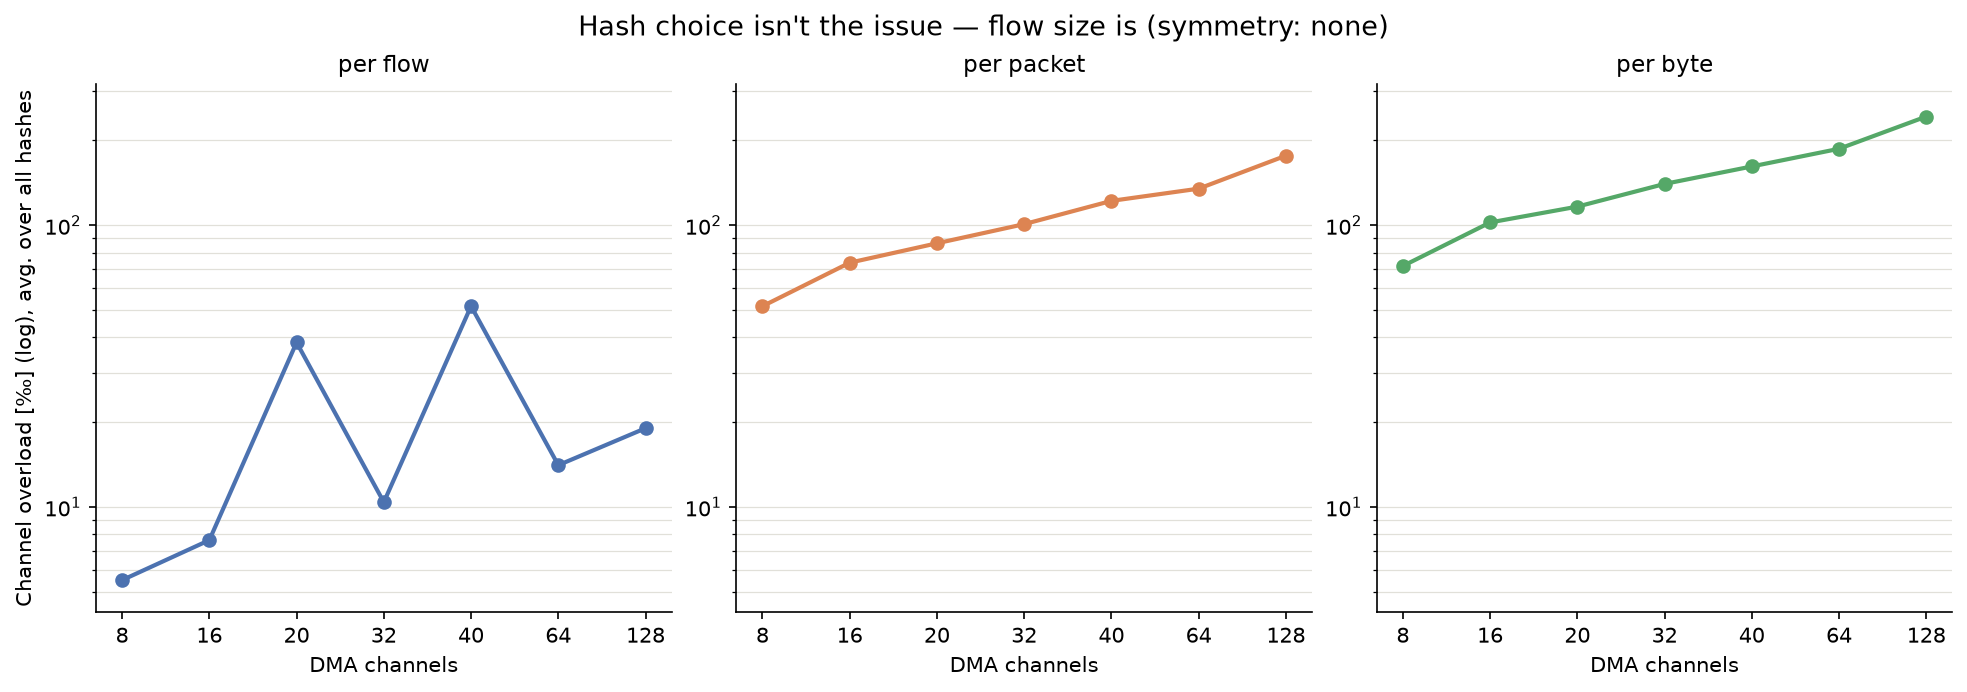
\includegraphics[width=\textwidth]{analyza/elephant_evidence.png}
  \caption{Preťaženie spriemerované cez všetky hashe pri troch váhach (logaritmická os).
  Špičky pri 20 a 40 kanáloch vo váhe flow spôsobuje kvantizácia RETA.
  \TODO{Prekresliť so slovenskými popismi.}}
  \label{fig:slony}
\end{figure}

\section{Porovnanie hashovacích funkcií}
\label{sec:hash-nezalezi}

Porovnávalo sa päť funkcií: Toeplitz, jhash, Chaskey, HalfSipHash a jednoduchá tabelácia.
Každá so 16 kľúčmi, tromi režimami symetrie, tromi váhami a siedmimi počtami kanálov, teda
5\,040 kombinácií na vzorke \texttt{odid1}.

% !TEX root = ../projekt.tex
\begin{table}[ht]
  \centering
  \small
  \caption{Preťaženie [\textperthousand] hashovacích funkcií na \texttt{odid1}: priemer cez 7 počtov kanálov, 16 kľúčov a všetky okná. Tučne je najnižšia hodnota v~riadku.}
  \label{tab:hashe-priemer}
  \begin{tabular}{l l rrrrr}
    \toprule
    Symetria & Váha & Toeplitz & jhash & Chaskey & HalfSipHash & simple tab. \\
    \midrule
    none & flow & \textbf{20,9} & 20,9 & 21,0 & 21,0 & 21,0 \\
    none & packet & 106,4 & 106,1 & \textbf{105,0} & 107,4 & 107,9 \\
    none & byte & 145,9 & 145,6 & \textbf{144,3} & 147,4 & 147,0 \\
    \midrule
    XOR & flow & 23,1 & 23,1 & 23,1 & 23,1 & \textbf{23,1} \\
    XOR & packet & 121,7 & 121,5 & 121,4 & 121,5 & \textbf{120,7} \\
    XOR & byte & 148,9 & 148,7 & 148,9 & 149,1 & \textbf{147,8} \\
    \midrule
    sort & flow & 23,1 & \textbf{23,1} & 23,2 & 23,2 & 23,1 \\
    sort & packet & 123,5 & 121,4 & \textbf{120,1} & 121,7 & 122,7 \\
    sort & byte & 151,6 & 148,5 & \textbf{146,8} & 149,5 & 149,9 \\
    \bottomrule
  \end{tabular}
\end{table}


Tabuľka~\ref{tab:hashe-priemer} ukazuje, že po spriemerovaní cez počty kanálov sú funkcie
veľmi blízko seba. Pri váhe \texttt{flow} sa líšia najviac o~0,1\,\textperthousand, pri váhach
\texttt{packet} a \texttt{byte} o~jednotky promile. Žiadna funkcia nie je najlepšia
vo všetkých režimoch.

% !TEX root = ../projekt.tex
\begin{table}[ht]
  \centering
  \small
  \caption{Odchýlka preťaženia od Toeplitzu na \texttt{odid1}. Záporná hodnota znamená lepší výsledok než Toeplitz.}
  \label{tab:hashe-odchylky}
  \begin{tabular}{l l r r l r}
    \toprule
    Symetria & Váha & priem. $|$odchýlka$|$ [\%] & najväčšia [\%] & funkcia & kanály \\
    \midrule
    none & flow & 0,5 & $+1{,}4$ & Chaskey & 16 \\
    none & packet & 1,6 & $-7{,}0$ & Chaskey & 8 \\
    none & byte & 1,2 & $-4{,}2$ & Chaskey & 8 \\
    \midrule
    XOR & flow & 0,6 & $+2{,}6$ & HalfSipHash & 8 \\
    XOR & packet & 0,8 & $+3{,}0$ & Chaskey & 8 \\
    XOR & byte & 0,7 & $+3{,}2$ & Chaskey & 8 \\
    \midrule
    sort & flow & 0,5 & $-1{,}3$ & jhash & 8 \\
    sort & packet & 2,1 & $-9{,}1$ & Chaskey & 16 \\
    sort & byte & 2,3 & $-8{,}4$ & Chaskey & 16 \\
    \bottomrule
  \end{tabular}
\end{table}


\subsection{Bez symetrie}

\begin{figure}[ht]
  \centering
  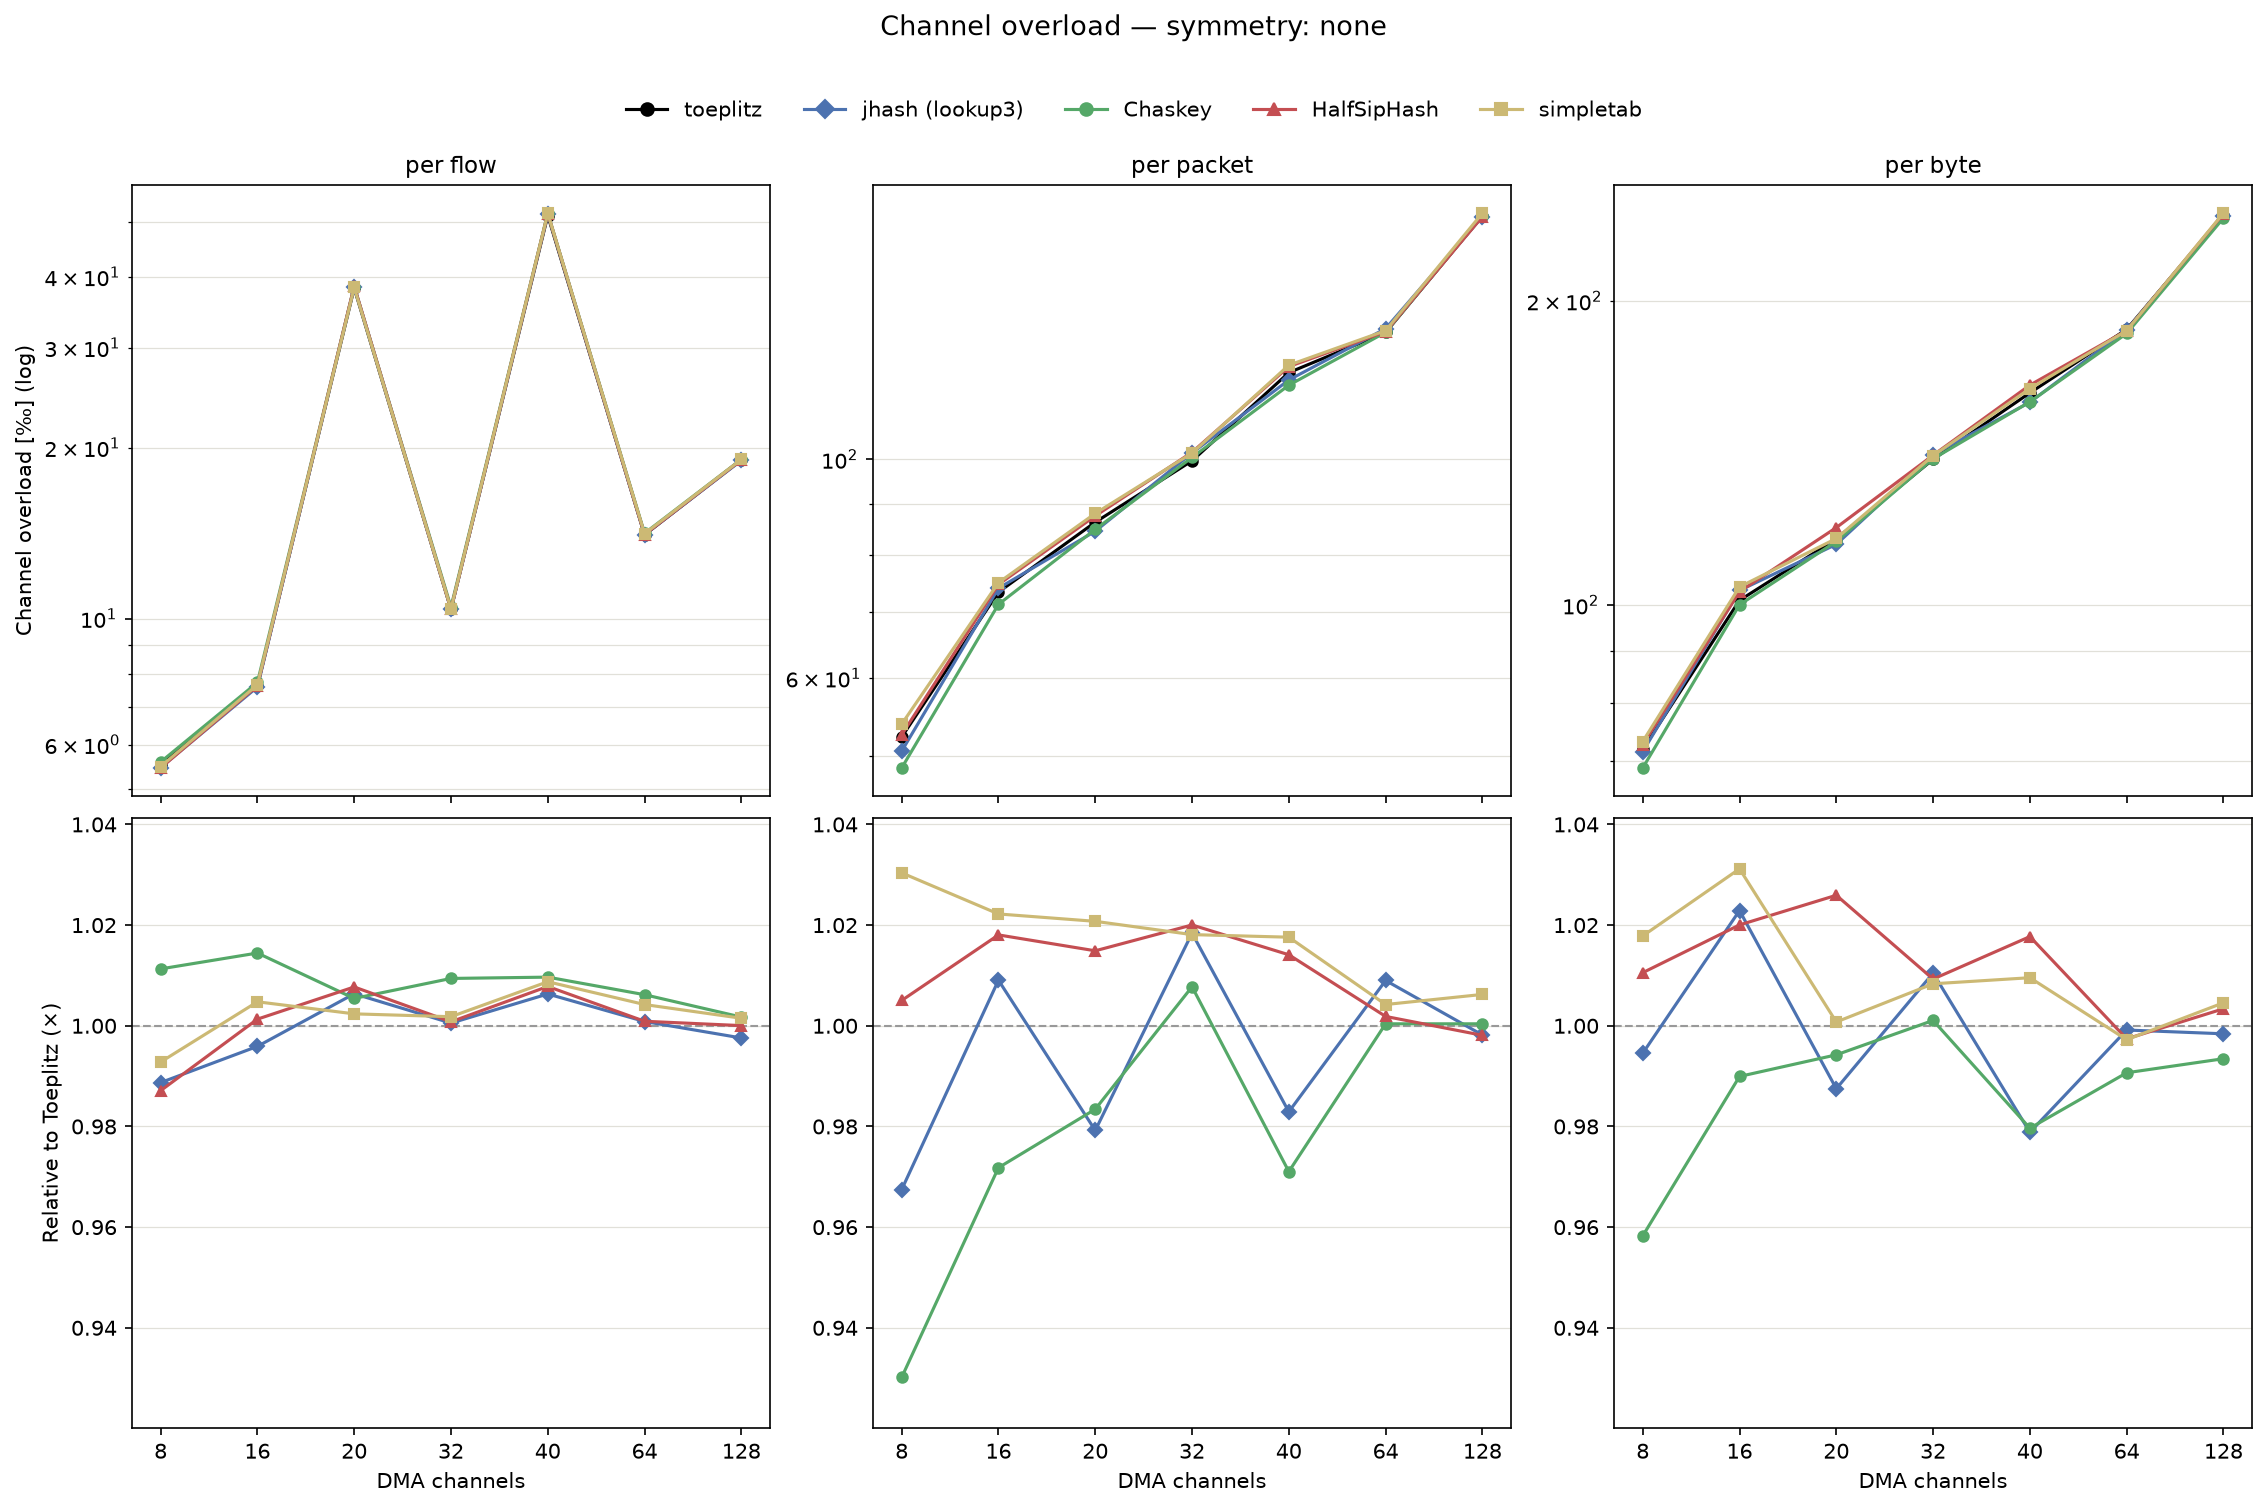
\includegraphics[width=\textwidth]{hashe/overload_none.png}
  \caption{Preťaženie piatich hashovacích funkcií bez symetrie (hore) a ich pomer
  k~Toeplitzu (dole), \texttt{odid1}. \TODO{Prekresliť so slovenskými popismi.}}
  \label{fig:hashe}
\end{figure}

Na obrázku~\ref{fig:hashe} sa krivky funkcií v~hornom riadku takmer prekrývajú. Spodný riadok
rozdiely zväčšuje: priemerná odchýlka od Toeplitzu je 0,5\,\% (flow), 1,6\,\% (packet)
a 1,2\,\% (byte). Najväčší rozdiel je pri 8 kanáloch a váhe \texttt{packet}, kde je Chaskey
o~7,0\,\% \emph{lepší} než Toeplitz. Väčšina odchýlok nemá stabilný smer: napríklad jhash je
pri váhe \texttt{packet} a 8 kanáloch lepší než Toeplitz, ale pri 16 kanáloch horší. Rozdiely sa navyše s~rastúcim počtom
kanálov zmenšujú a pri 128 kanáloch sú všetky funkcie do približne 1\,\% od Toeplitzu.

Pri váhe \texttt{flow} sú krivky prakticky totožné a výrazné špičky pri 20 a 40 kanáloch majú
všetky funkcie rovnaké, lebo ich spôsobuje RETA (sekcia~\ref{sec:reta}).

\subsection{Symetria XOR}

\begin{figure}[ht]
  \centering
  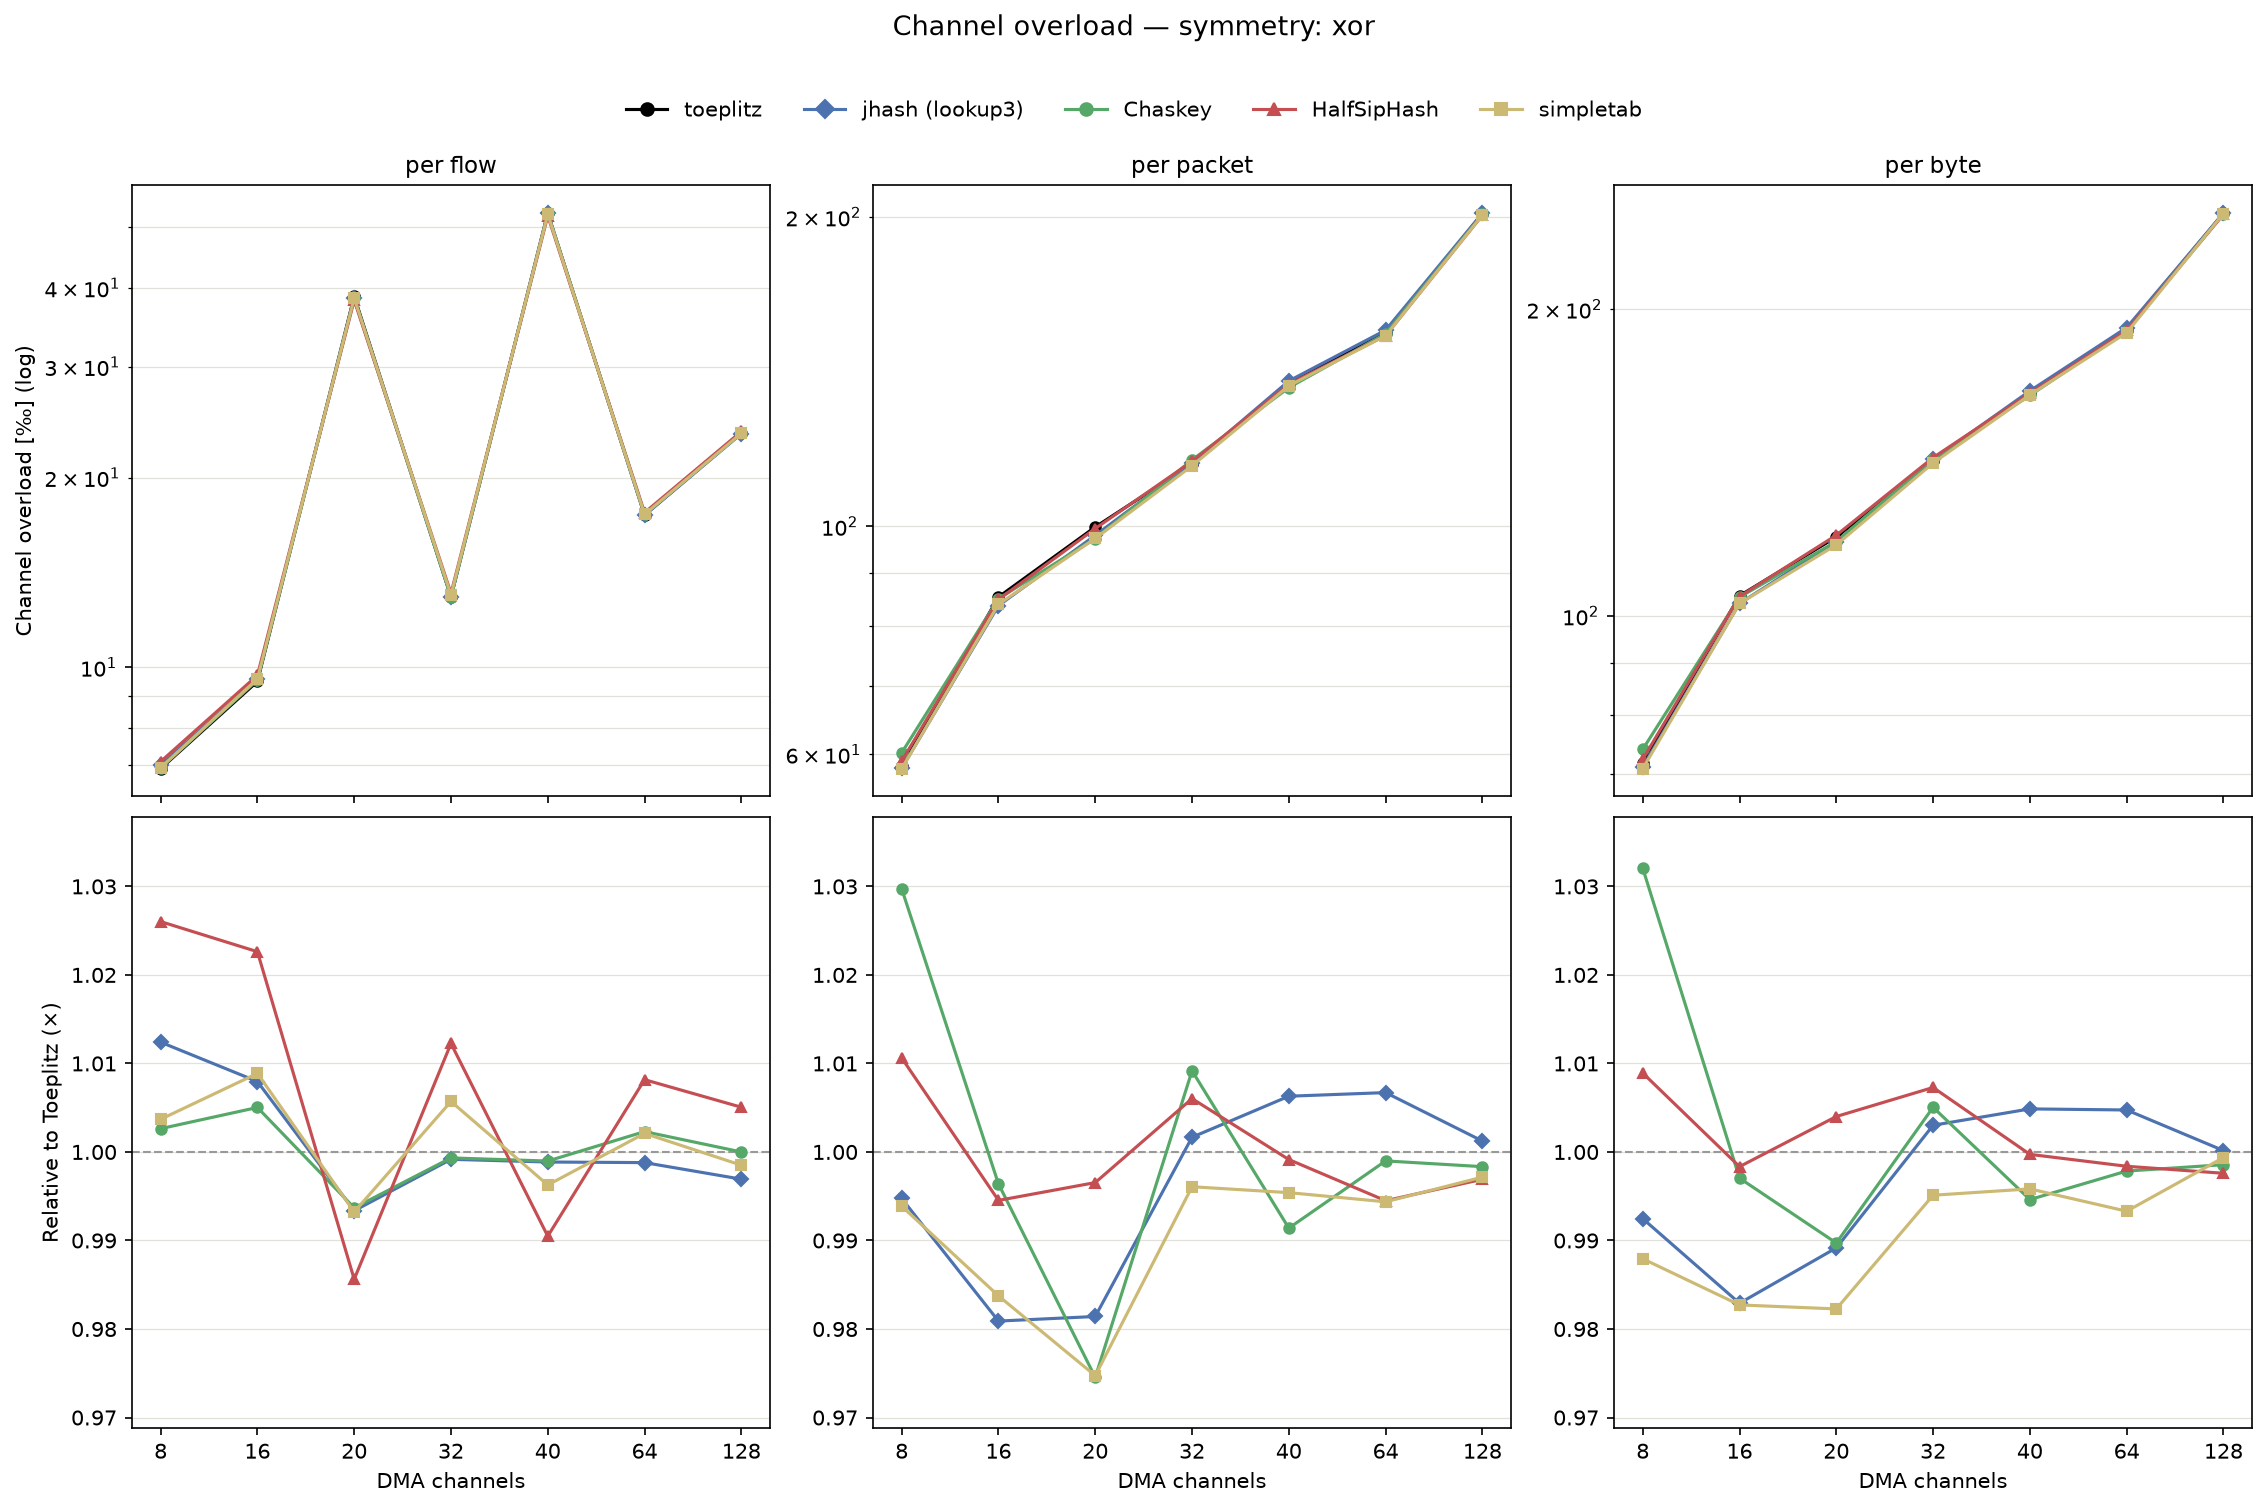
\includegraphics[width=\textwidth]{hashe/overload_xorfold.png}
  \caption{Porovnanie funkcií pri symetrii XOR, \texttt{odid1}.
  \TODO{Prekresliť so slovenskými popismi.}}
  \label{fig:hashe-xor}
\end{figure}

Pri symetrii XOR (obrázok~\ref{fig:hashe-xor}) sú funkcie najbližšie k~sebe. Priemerná
odchýlka je 0,6 až 0,8\,\% a najväčšia 3,2\,\%.

\subsection{Symetria sort}

\begin{figure}[ht]
  \centering
  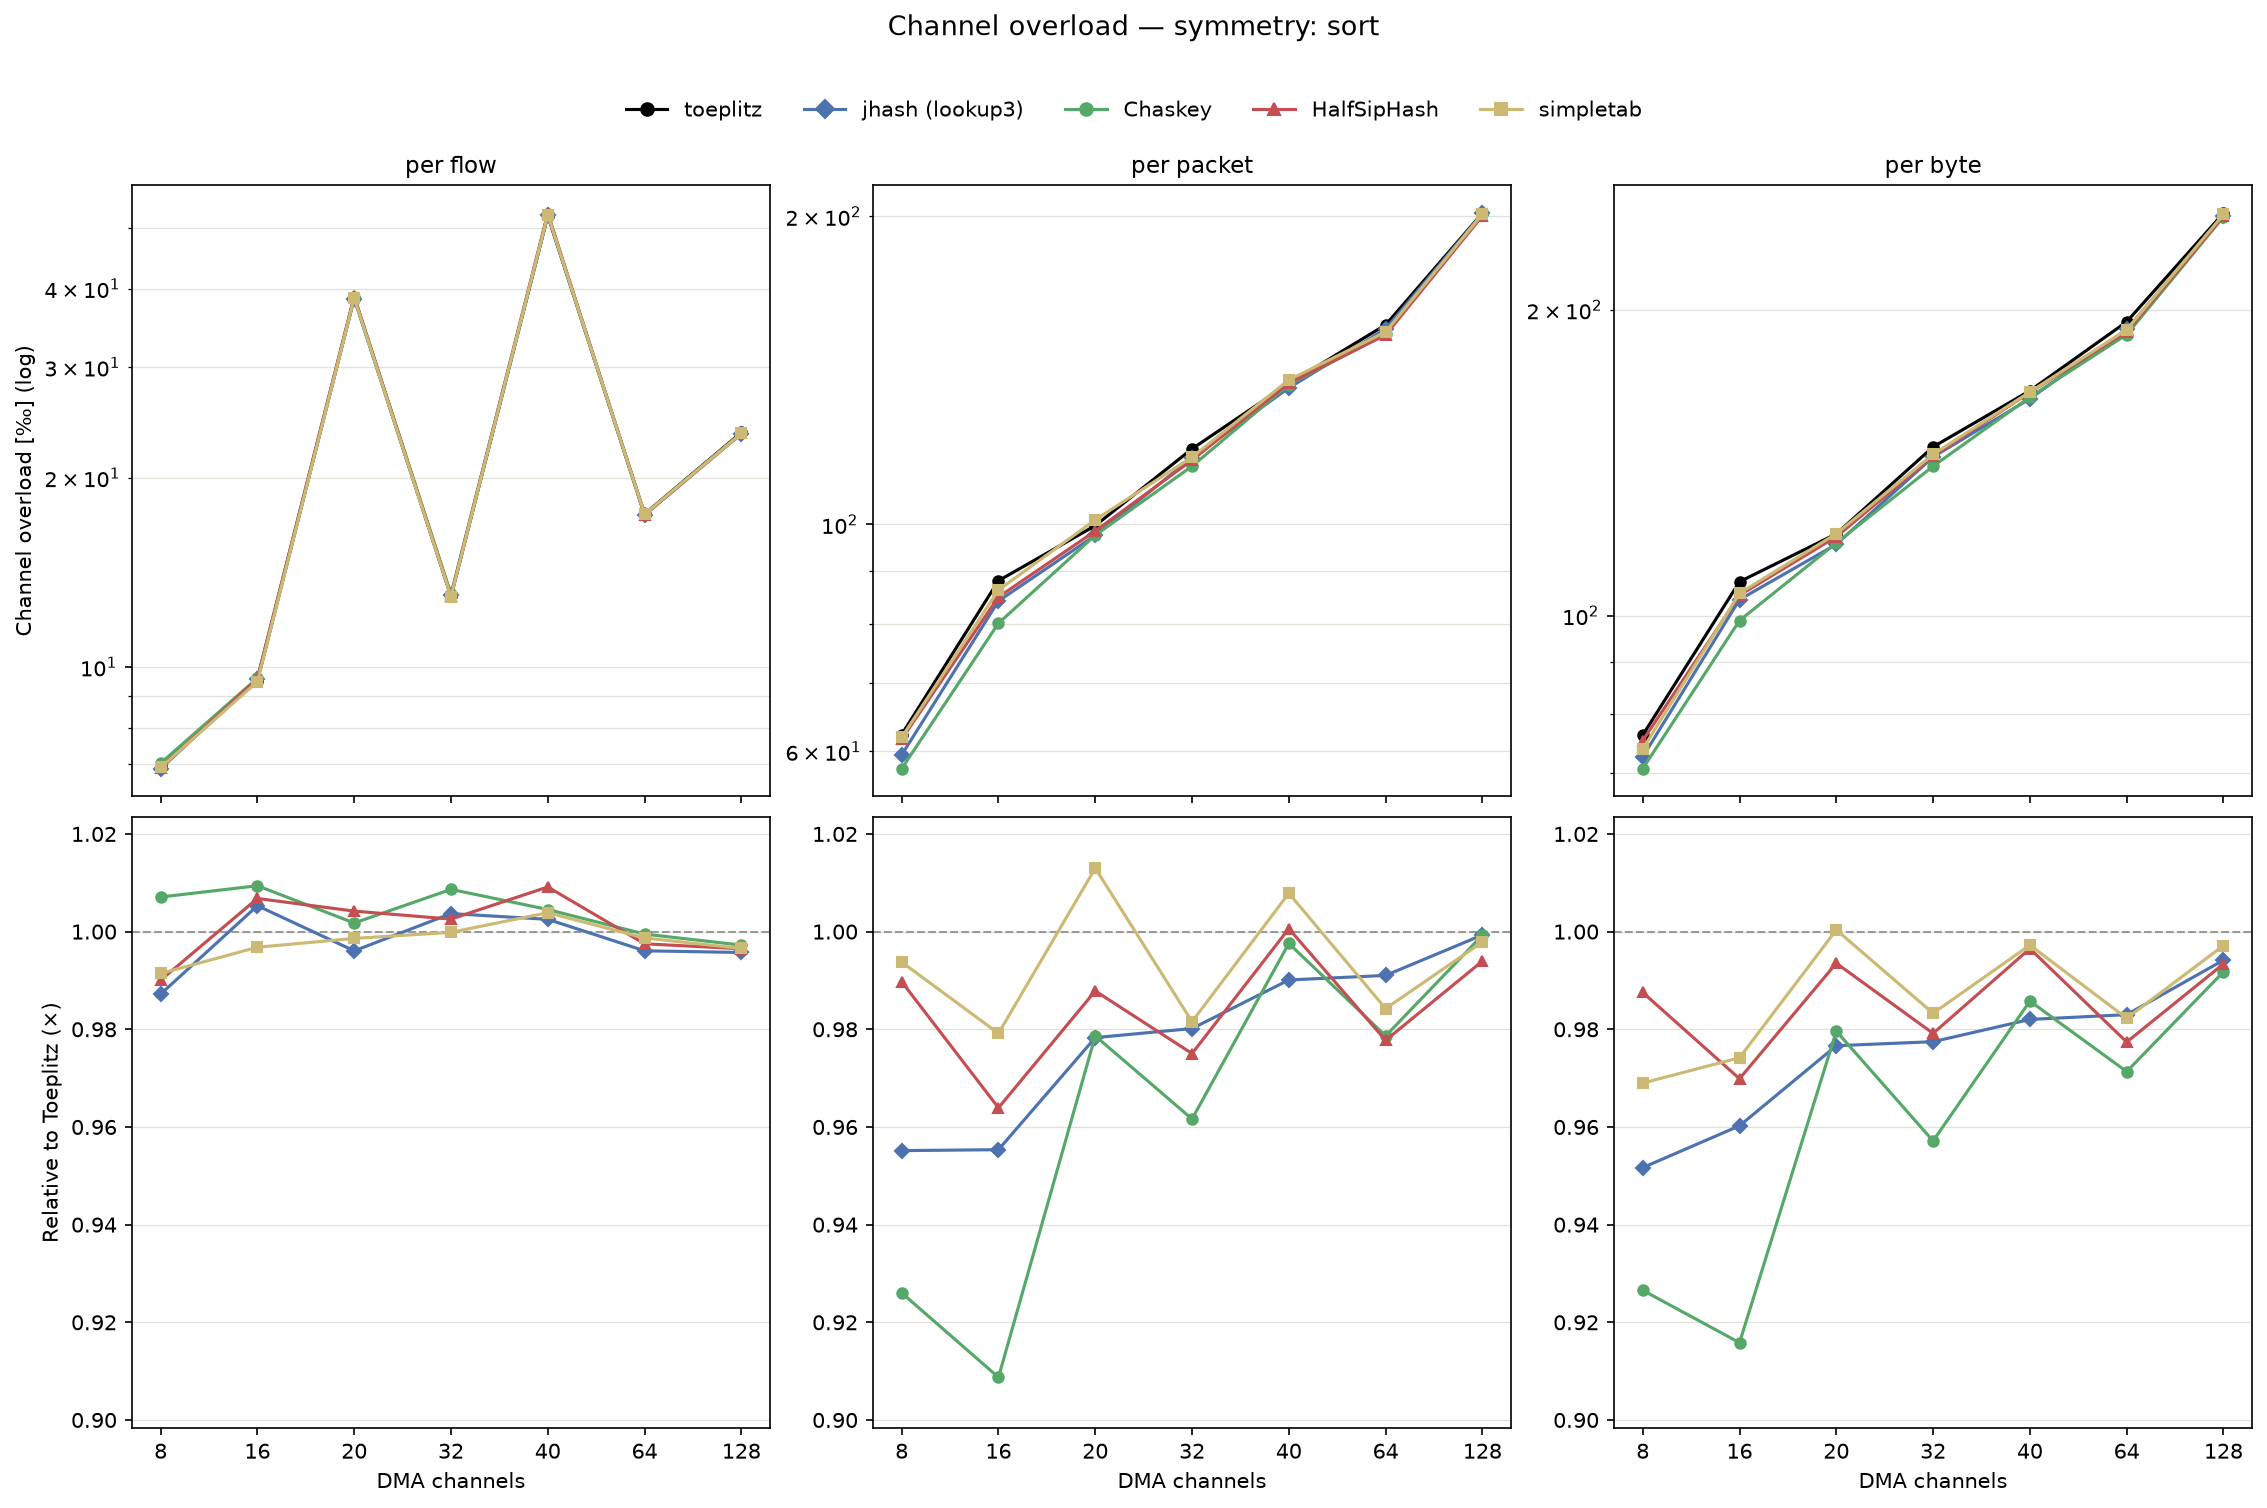
\includegraphics[width=\textwidth]{hashe/overload_sortfold.png}
  \caption{Porovnanie funkcií pri symetrii sort, \texttt{odid1}.
  \TODO{Prekresliť so slovenskými popismi.}}
  \label{fig:hashe-sort}
\end{figure}

Symetria sort je jediný režim, kde sa objavuje náznak systematického rozdielu
(obrázok~\ref{fig:hashe-sort}). Pri váhach \texttt{packet} a \texttt{byte} má Toeplitz
v~priemere najvyššie preťaženie a ostatné funkcie sú pri väčšine počtov kanálov pod ním. Chaskey
je pri 16 kanáloch lepší až o~9,1\,\%. Rozdiel sa s~rastúcim počtom kanálov opäť stráca.
\TODO{Overiť väčším počtom kľúčov, či je to skutočný efekt kombinácie Toeplitz + sort, alebo
náhoda. Toeplitz je lineárny, takže tu môže existovať vysvetlenie.}

\section{Vplyv RSS kľúča}
\label{sec:kluce}

Aby sa dalo posúdiť, či sú rozdiely medzi funkciami významné, treba ich porovnať s~tým, ako
veľmi sa mení výsledok \emph{tej istej} funkcie pri inom náhodnom kľúči.

% !TEX root = ../projekt.tex
\begin{table}[ht]
  \centering
  \small
  \caption{Vplyv kľúča bez symetrie, \texttt{odid1}, hodnoty v~\textperthousand. \emph{Toeplitz}: najlepší až najhorší zo 16 kľúčov. \emph{Hashe}: rozpätie priemerov piatich funkcií. \emph{Kľúče}: priemerné rozpätie medzi kľúčmi jednej funkcie.}
  \label{tab:kluce}
  \begin{tabular}{r rrrr rrrr}
    \toprule
    & \multicolumn{4}{c}{packet} & \multicolumn{4}{c}{byte} \\
    Kanály & Toeplitz & hashe & kľúče & pomer & Toeplitz & hashe & kľúče & pomer \\
    \midrule
    8 & 41,9--71,3 & 5,2 & 21,0 & 4,0$\times$ & 60,1--96,0 & 4,3 & 27,9 & 6,5$\times$ \\
    16 & 61,0--83,1 & 3,7 & 18,5 & 5,0$\times$ & 86,8--116,0 & 4,2 & 26,2 & 6,3$\times$ \\
    20 & 75,9--95,5 & 3,6 & 20,9 & 5,8$\times$ & 101,7--128,3 & 4,5 & 25,6 & 5,7$\times$ \\
    32 & 91,6--108,4 & 2,0 & 16,6 & 8,3$\times$ & 128,8--151,1 & 1,5 & 21,1 & 14,4$\times$ \\
    40 & 106,2--133,4 & 5,7 & 22,2 & 3,9$\times$ & 140,7--173,4 & 6,3 & 29,0 & 4,6$\times$ \\
    64 & 127,9--143,2 & 1,2 & 15,0 & 12,4$\times$ & 178,2--201,0 & 1,7 & 20,2 & 11,6$\times$ \\
    128 & 170,2--183,5 & 1,4 & 12,6 & 8,8$\times$ & 235,8--251,0 & 2,7 & 15,4 & 5,7$\times$ \\
    \bottomrule
  \end{tabular}
\end{table}


Tabuľka~\ref{tab:kluce} ukazuje, že kľúč má väčší vplyv než výber funkcie pri každom počte
kanálov: rozpätie medzi kľúčmi je 3,9 až 12,4-krát väčšie pri váhe \texttt{packet} a 4,6 až
14,4-krát pri váhe \texttt{byte}. Pri malom počte kanálov je vplyv kľúča veľký aj absolútne.
Toeplitz s~8 kanálmi má pri váhe \texttt{packet} podľa kľúča preťaženie od 41,9 do
71,3\,\textperthousand, teda jeho najhorší kľúč je o~70\,\% horší než najlepší. Pravdepodobným dôvodom je, že pri
málo kanáloch rozhoduje, či najväčšie toky padnú do toho istého kanála.
\TODO{Overiť: pozrieť, kam padnú najväčšie toky pri najlepšom a najhoršom kľúči.}

\begin{figure}[p]
  \centering
  \begin{subfigure}{0.54\textwidth}
    \centering
    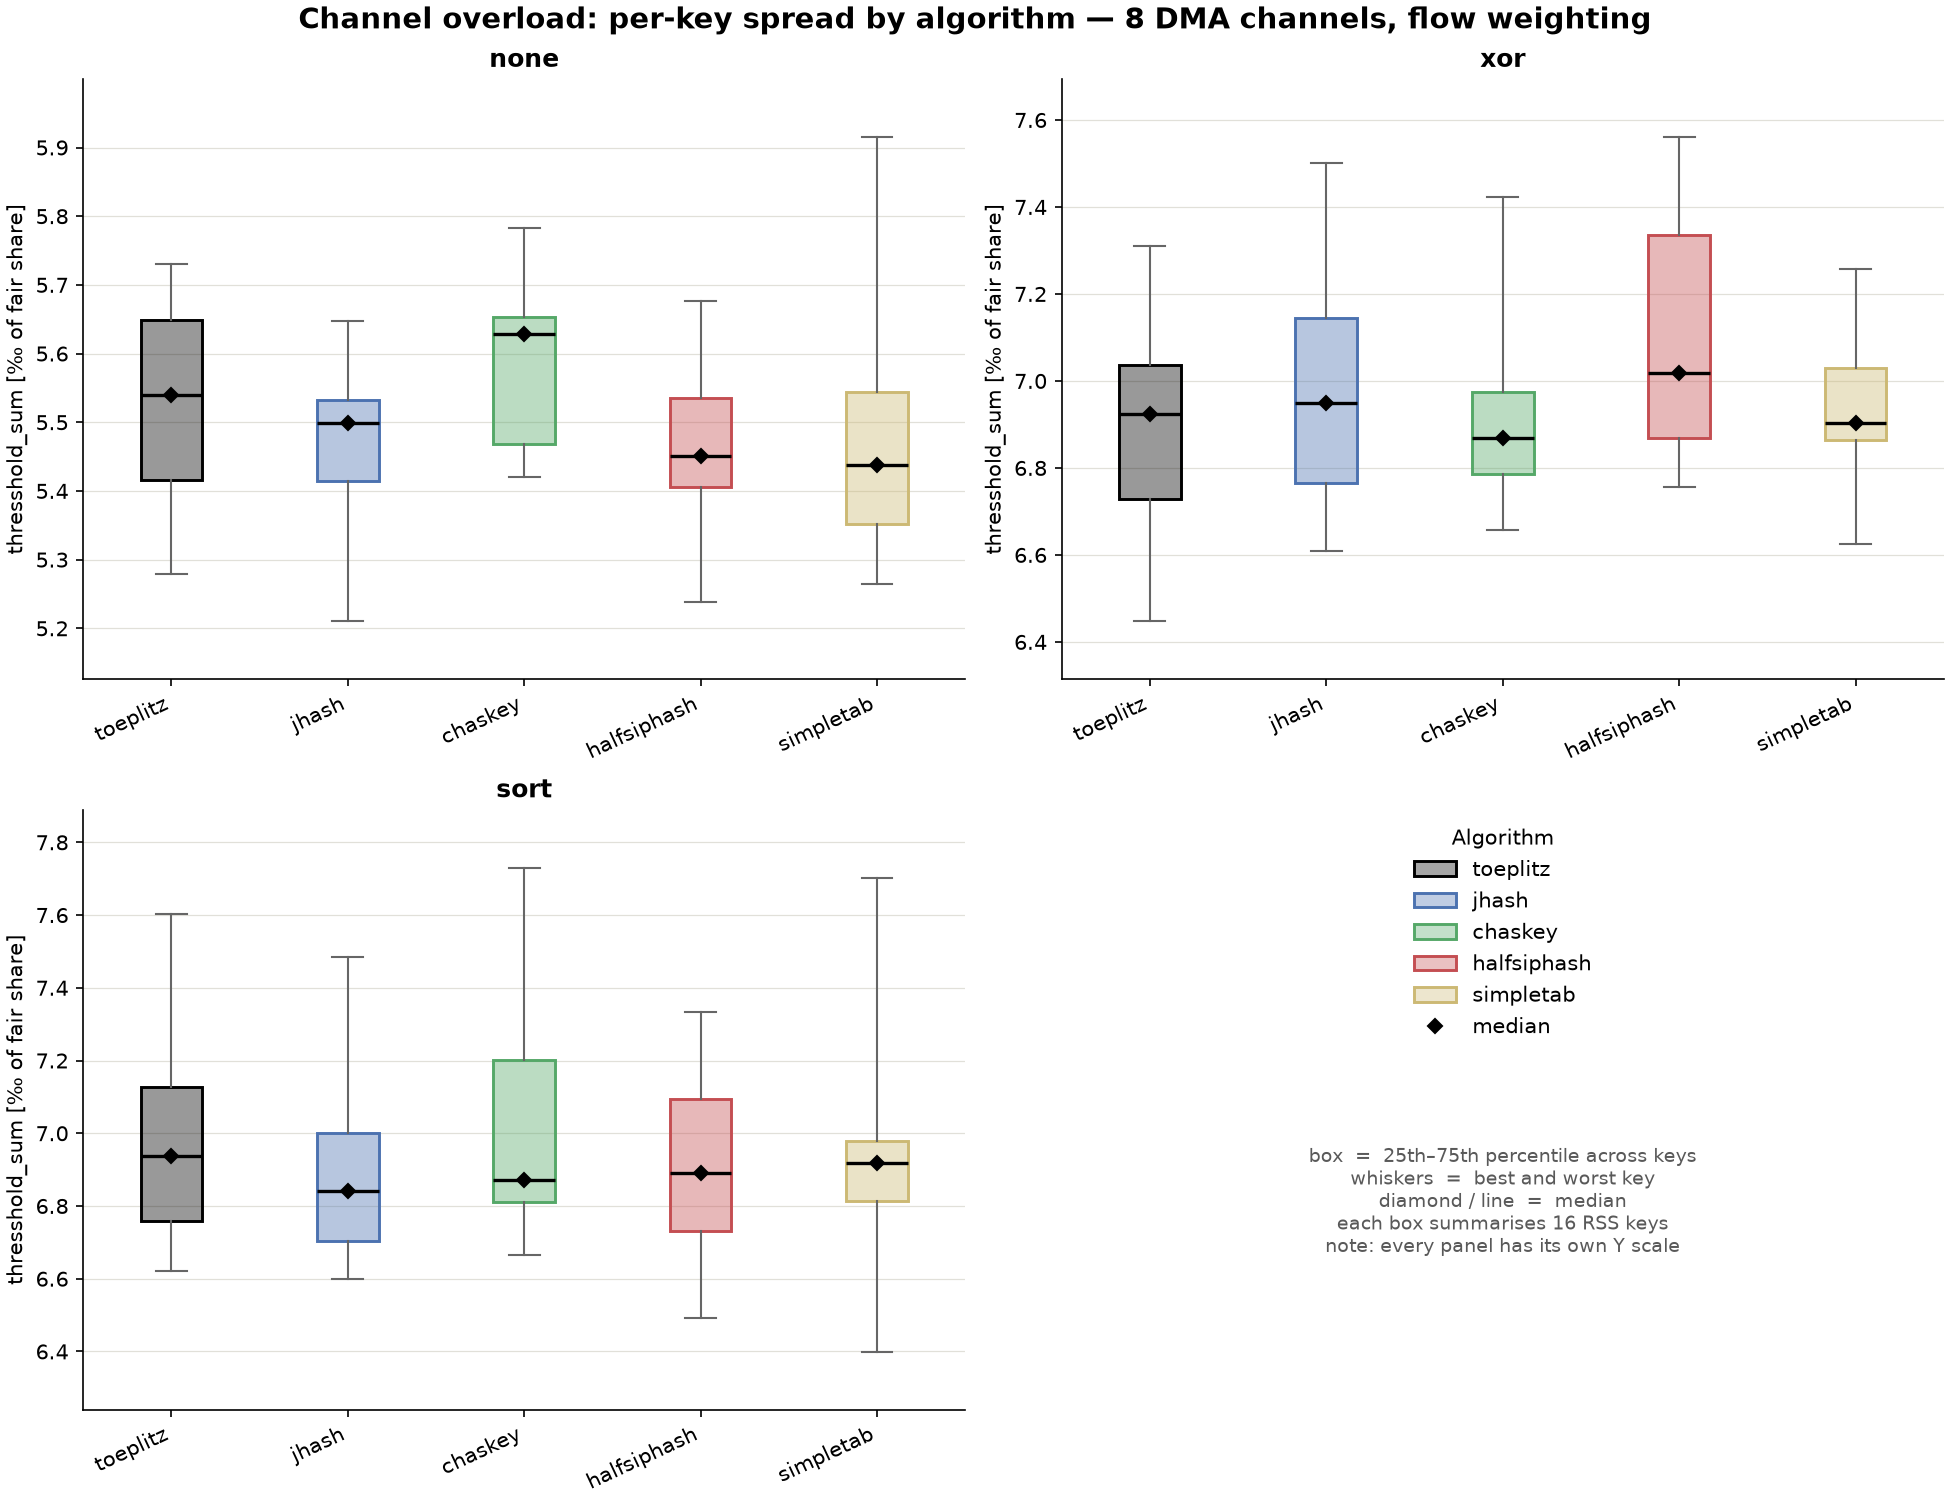
\includegraphics[width=\textwidth]{kluce/keys_8.png}
    \caption{8 kanálov}
  \end{subfigure}

  \begin{subfigure}{0.54\textwidth}
    \centering
    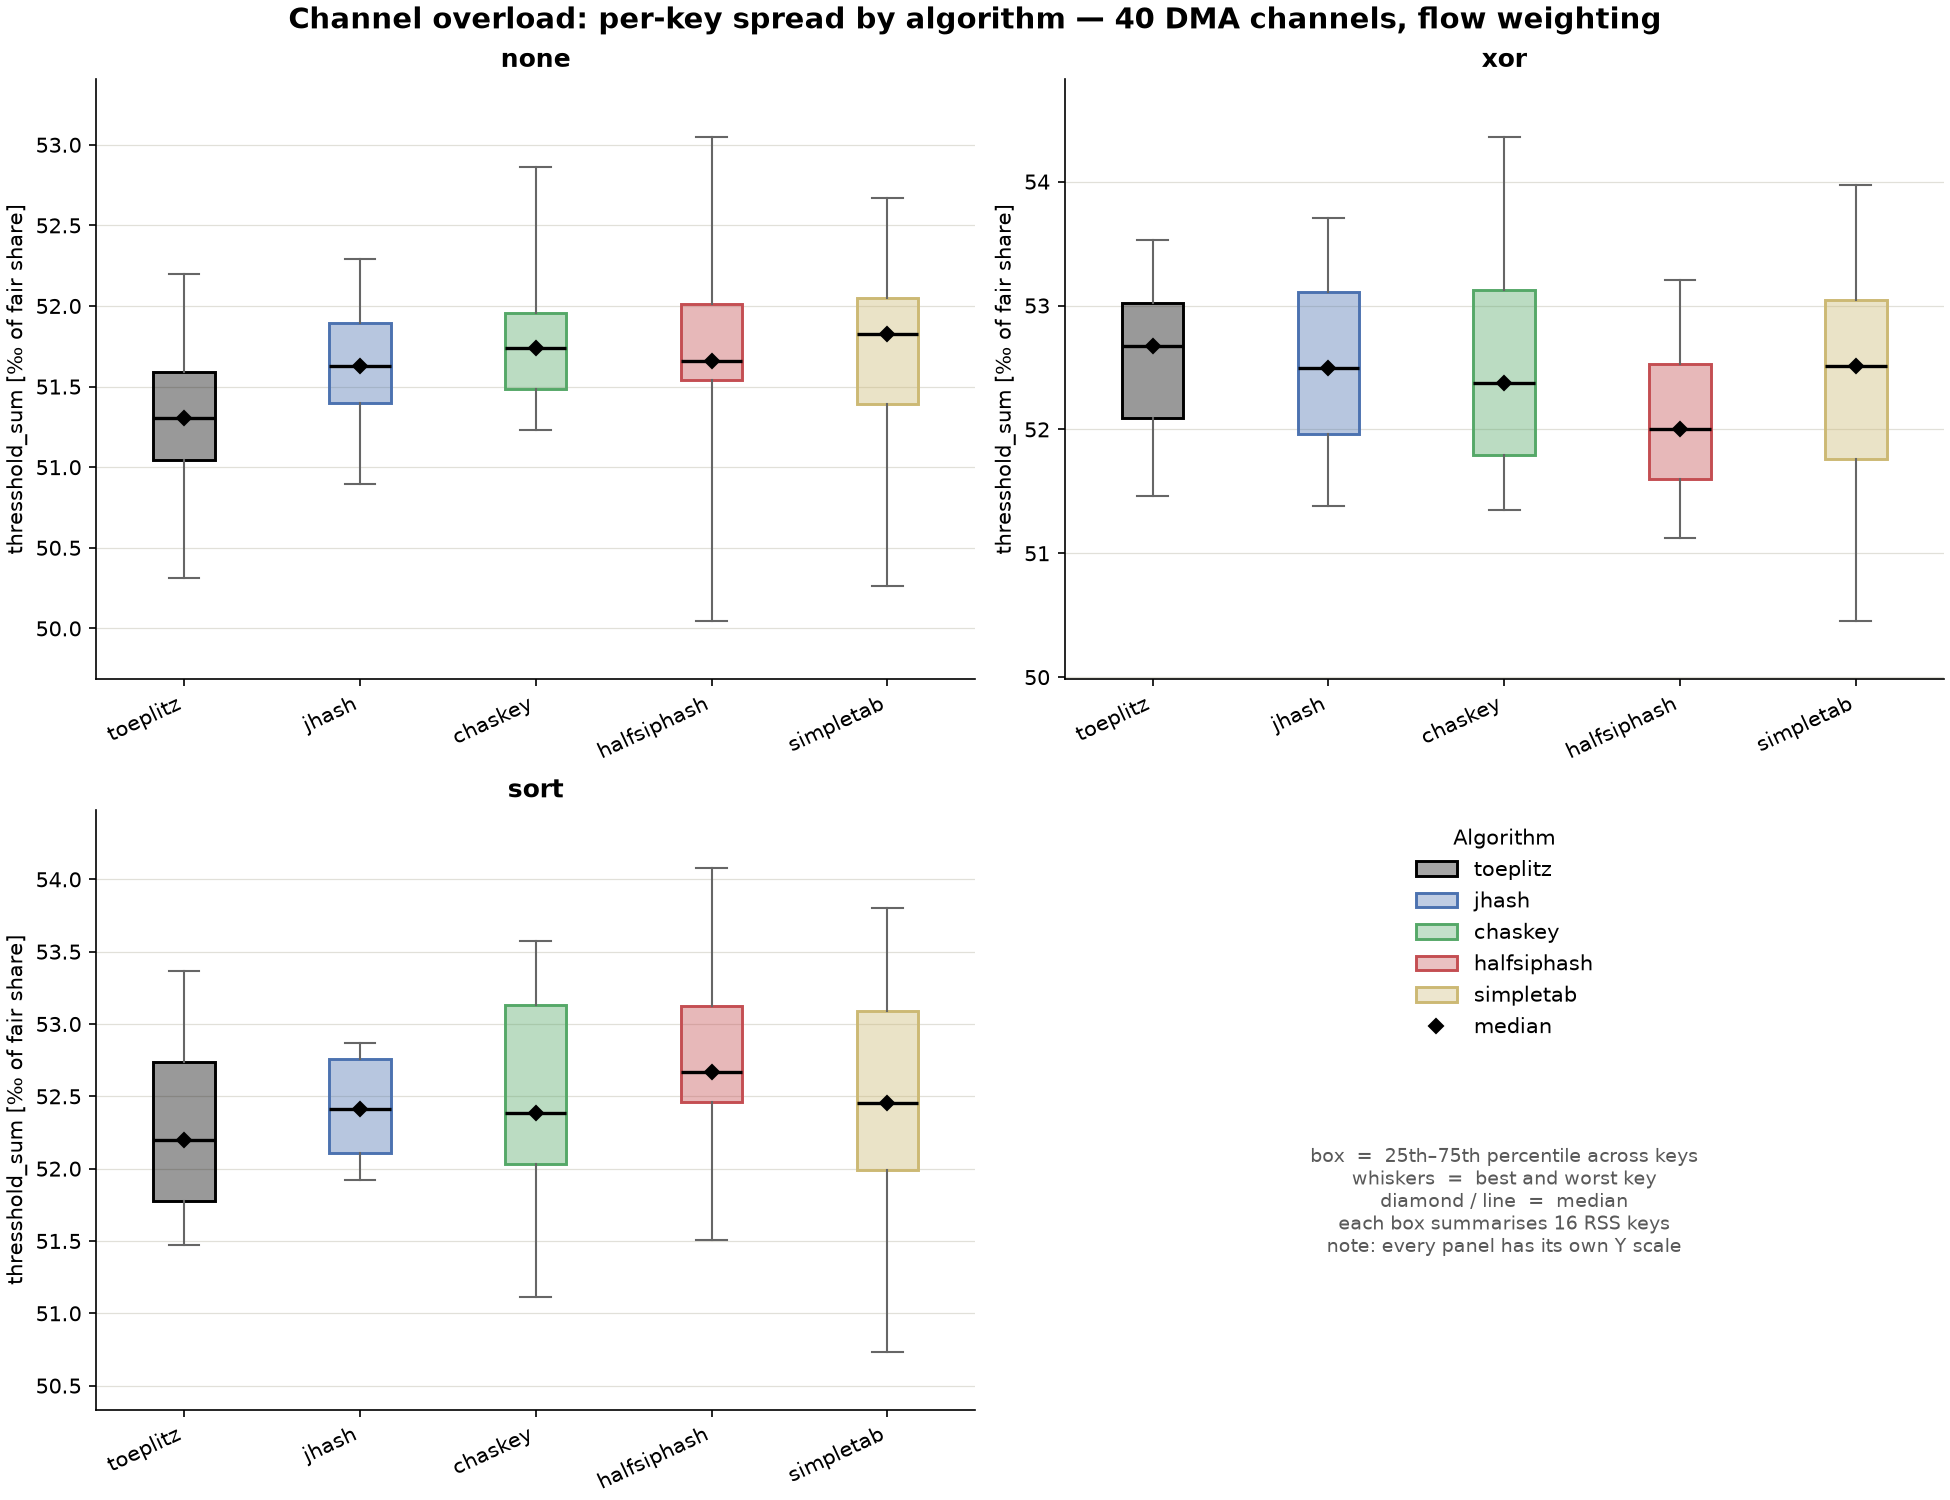
\includegraphics[width=\textwidth]{kluce/keys_40.png}
    \caption{40 kanálov}
  \end{subfigure}

  \begin{subfigure}{0.54\textwidth}
    \centering
    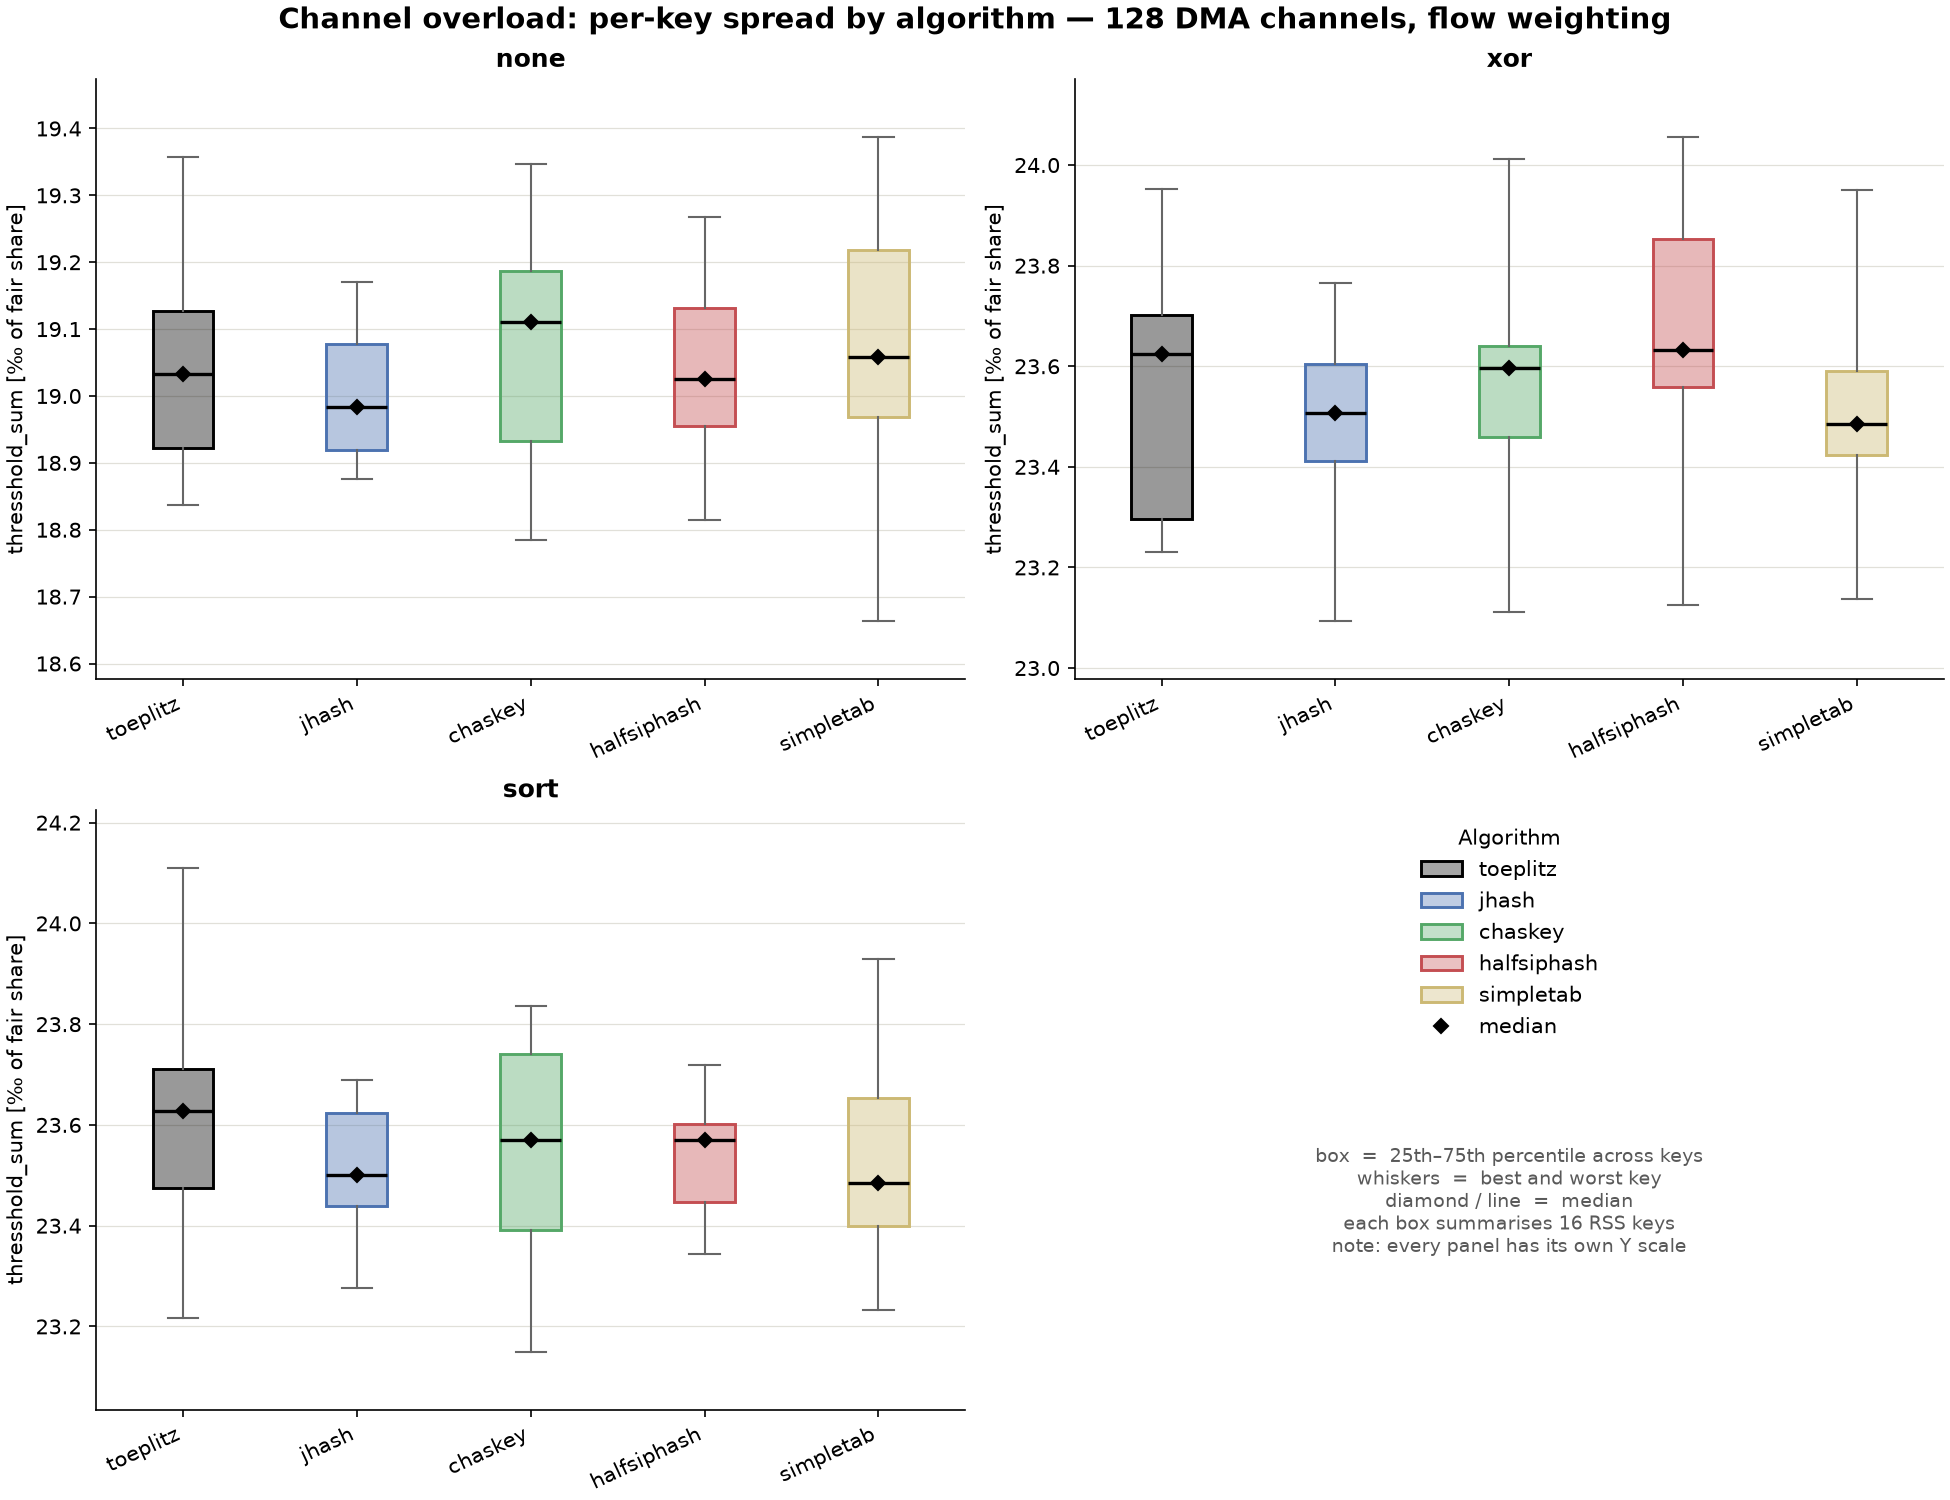
\includegraphics[width=\textwidth]{kluce/keys_128.png}
    \caption{128 kanálov}
  \end{subfigure}
  \caption{Rozptyl preťaženia medzi 16 kľúčmi pri váhe \texttt{flow}, \texttt{odid1}. Škatuľa
  je 25.--75.~percentil, fúzy sú najlepší a najhorší kľúč. Každý panel má vlastnú os Y.
  \TODO{Prekresliť so slovenskými popismi.}}
  \label{fig:kluce}
\end{figure}

Obrázok~\ref{fig:kluce} zobrazuje rozloženie cez kľúče pri váhe \texttt{flow}, kde sa meria čistá
kvalita hashu bez vplyvu veľkých tokov. Škatule všetkých funkcií sa vo všetkých režimoch
prekrývajú, takže podľa rozloženia cez kľúče nemožno žiadnu funkciu označiť za lepšiu.
Pozor na mierku: pri 8 kanáloch je celý rozsah Toeplitzu bez symetrie iba 5,3 až
5,7\,\textperthousand{} a pri 128 kanáloch 18,8 až 19,4\,\textperthousand.

\emph{Poznámka:} výber ,,najlepšieho`` kľúča na tých istých dátach by bol zavádzajúci. Dobrý
kľúč je výhodný preto, ako práve rozdelil konkrétne veľké toky, a na inej prevádzke výhodu stratí.
\TODO{Dalo by sa overiť: vybrať najlepší kľúč na jednej vzorke a zmerať ho na inej.}

\section{Štatistické vyhodnotenie}
\label{sec:statistika}

\begin{itemize}
  \item \textbf{Kľúč oproti funkcii.} Cez všetkých 63 konfigurácií (3 symetrie, 3 váhy, 7 počtov
        kanálov) je rozpätie medzi kľúčmi v~mediáne 6,6-krát väčšie než rozpätie medzi
        funkciami (od 3,1 do 23,1-krát).
  \item \textbf{Permutačný test.} Hodnoty kľúčov sme náhodne premiešali medzi funkciami
        (3\,000 permutácií) a testovali, či je skutočný rozdiel funkcií väčší než náhodný.
        $p<0{,}05$ vyšlo v~4 z~63 konfigurácií, čisto náhodou by sa očakávali približne 3.
        Žiadna konfigurácia nemá $p<0{,}01$. Všetky štyri sú pri symetrii \emph{sort}, čo
        zodpovedá náznaku z~obrázka~\ref{fig:hashe-sort}.
  \item \textbf{Podiel vysvetleného rozptylu.} Voľba funkcie vysvetľuje najviac približne
        14\,\% rozptylu výsledkov ($\eta^2$, obrázok~\ref{fig:spread}), väčšinou menej než 10\,\%.
\end{itemize}

\begin{figure}[ht]
  \centering
  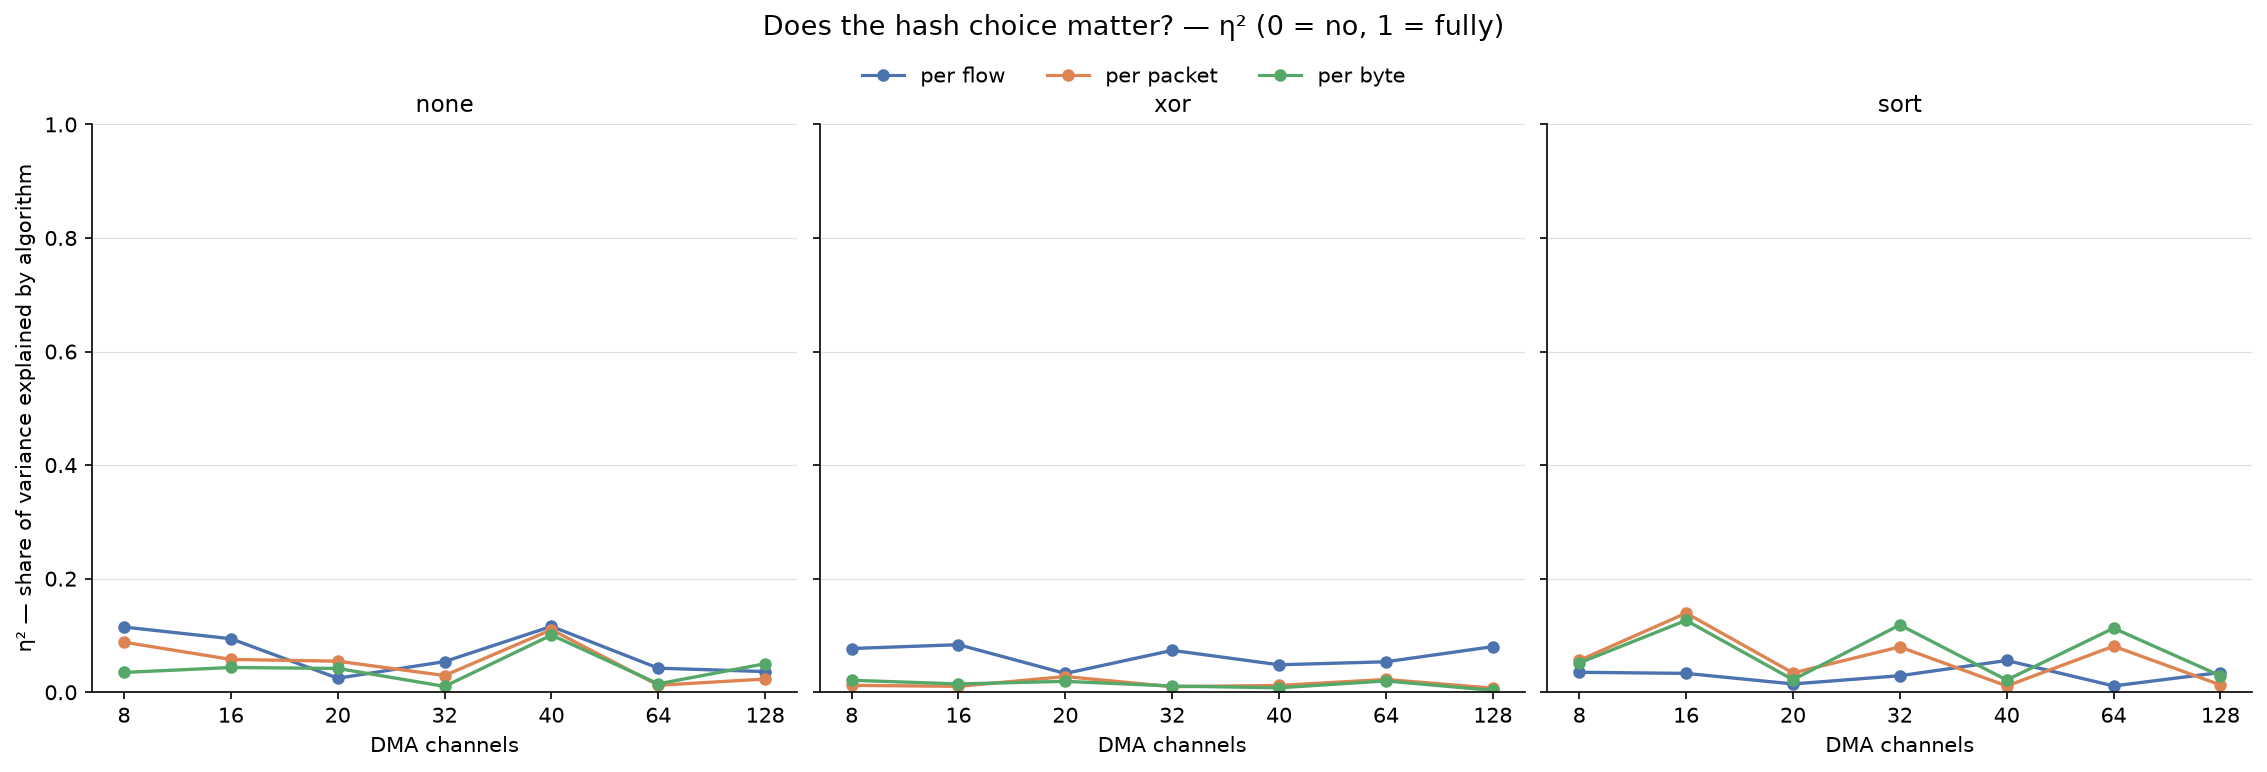
\includegraphics[width=\textwidth]{hashe/spread.png}
  \caption{Podiel rozptylu vysvetlený voľbou hashovacej funkcie ($\eta^2$), \texttt{odid1}.
  \TODO{Prekresliť so slovenskými popismi.}}
  \label{fig:spread}
\end{figure}

\paragraph{Záver porovnania.} Na vzorke \texttt{odid1} s~plným tuple sa medzi piatimi funkciami
nepreukázal rozdiel, ktorý by prevýšil vplyv náhodného kľúča. Výmena kvalitného hashu preto
nerieši nerovnomernú záťaž. Sekcia~\ref{sec:dalsie-vzorky} ukazuje dôležitú výnimku:
slabšia funkcia môže byť horšia, keď má vstup málo entropie. Ďalšie experimenty používajú Toeplitz.

\section{Cena symetrie}
\label{sec:cena-symetrie}

% !TEX root = ../projekt.tex
\begin{table}[ht]
  \centering
  \small
  \caption{Zmena preťaženia Toeplitzu po zapnutí symetrie oproti \texttt{none}, cez 7 počtov kanálov.}
  \label{tab:symetria}
  \begin{tabular}{l rr rr}
    \toprule
    & \multicolumn{2}{c}{XOR} & \multicolumn{2}{c}{sort} \\
    Váha & priemer [\%] & rozsah [\%] & priemer [\%] & rozsah [\%] \\
    \midrule
    flow & +18,1 & +1,5 až +25,0 & +18,3 & +1,3 až +26,3 \\
    packet & +14,3 & +11,8 až +16,4 & +16,7 & +12,2 až +20,1 \\
    byte & +2,0 & -0,4 až +3,6 & +4,4 & +2,4 až +6,9 \\
    \bottomrule
  \end{tabular}
\end{table}


Symetria zlúči oba smery spojenia do jedného kanála, čím vznikajú väčšie jednotky záťaže.
Podľa tabuľky~\ref{tab:symetria} zvyšuje preťaženie pri váhach \texttt{flow} a \texttt{packet}
priemerne o~14 až 18\,\%, pri váhe \texttt{byte} iba o~2 až 4\,\%.
\TODO{Vysvetliť, prečo je cena pri bajtoch nižšia. Hypotéza: bajty sú v~jednom smere toku,
ten druhý k~záťaži pridá málo. Treba overiť na dátach.}

\section{Vplyv tabuľky RETA}

Pri 20 a 40 kanáloch tvorí preťaženie vo váhe \texttt{flow} takmer výlučne kvantizácia RETA
(sekcia~\ref{sec:reta}): teoreticky 37,5 a 50,0\,\textperthousand, namerané 38,2 a
51,3\,\textperthousand. Pri mocninách dvoch tento efekt neexistuje.

\section{Koľko sa dá získať pri zachovaní afinity toku}
\label{sec:hranica}

% !TEX root = ../projekt.tex
\begin{table}[ht]
  \centering
  \small
  \caption{Preťaženie [\textperthousand]: Toeplitz a orákulum JSQ, pevné okno, \texttt{odid1}.}
  \label{tab:jsq}
  \begin{tabular}{r rrr rrr}
    \toprule
    & \multicolumn{3}{c}{packet} & \multicolumn{3}{c}{byte} \\
    Kanály & Toeplitz & JSQ & zmena & Toeplitz & JSQ & zmena \\
    \midrule
    8 & 52,3 & 6,1 & $-88$\,\% & 72,0 & 12,0 & $-83$\,\% \\
    16 & 73,3 & 12,1 & $-84$\,\% & 101,0 & 22,8 & $-77$\,\% \\
    20 & 86,3 & 14,4 & $-83$\,\% & 116,3 & 26,8 & $-77$\,\% \\
    32 & 99,6 & 20,8 & $-79$\,\% & 139,4 & 35,8 & $-74$\,\% \\
    40 & 122,4 & 22,9 & $-81$\,\% & 162,2 & 41,0 & $-75$\,\% \\
    64 & 134,4 & 32,2 & $-76$\,\% & 187,4 & 54,8 & $-71$\,\% \\
    128 & 176,5 & 50,3 & $-71$\,\% & 243,2 & 89,4 & $-63$\,\% \\
    \bottomrule
  \end{tabular}
\end{table}


\begin{figure}[ht]
  \centering
  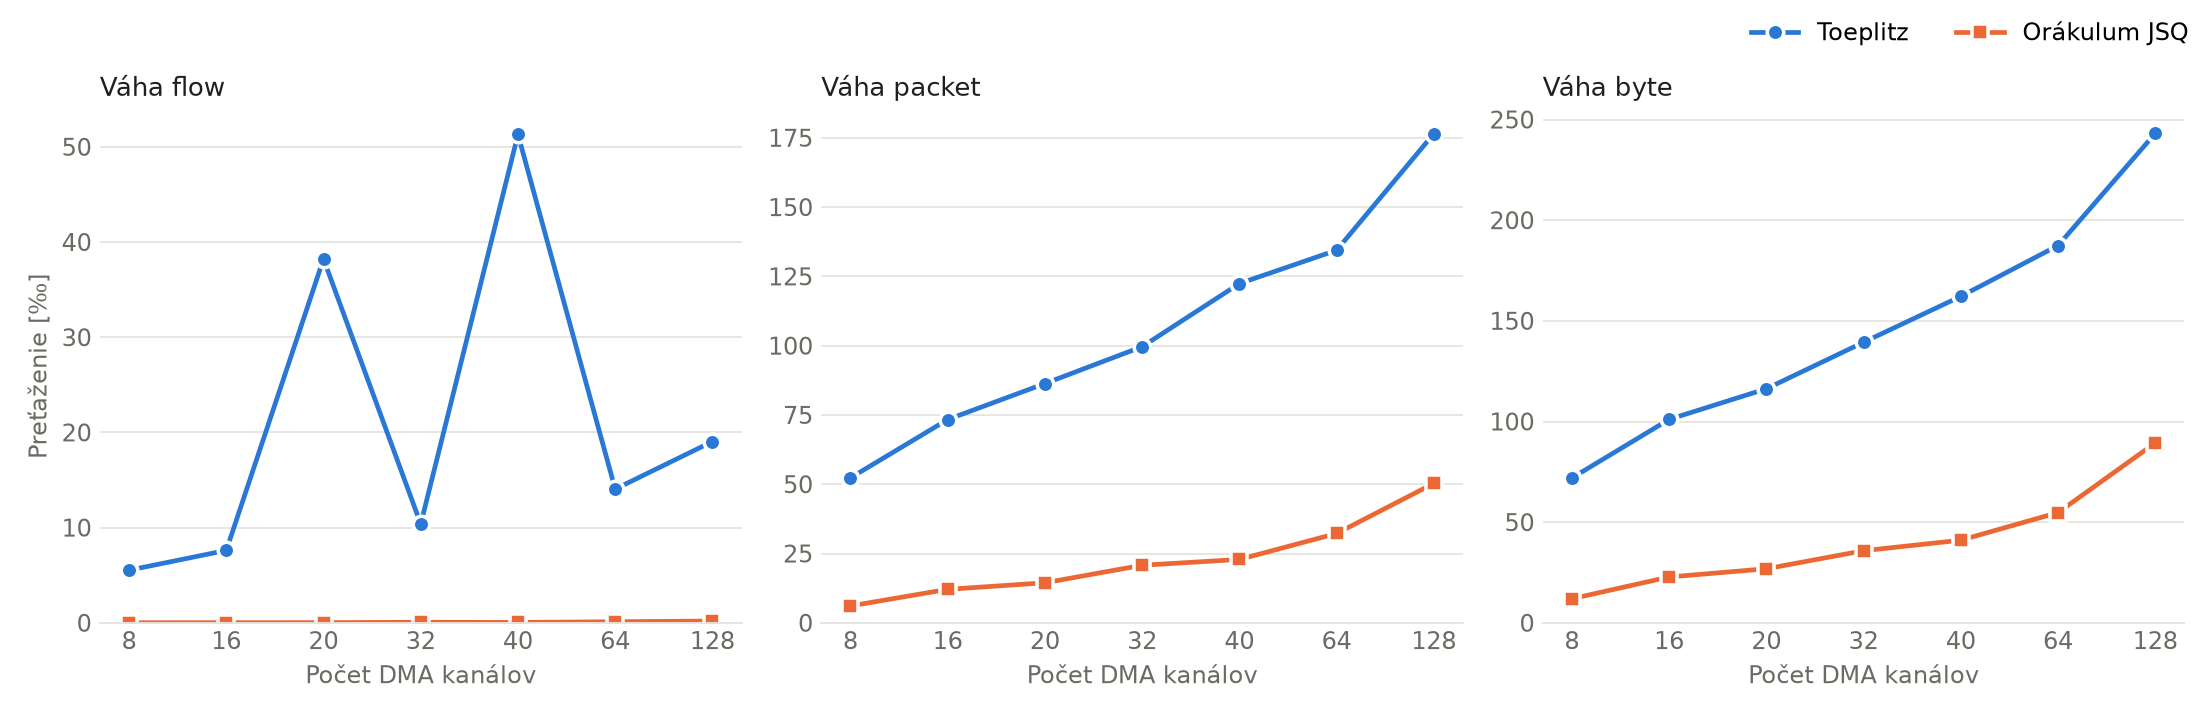
\includegraphics[width=\textwidth]{analyza/jsq_vs_toeplitz.png}
  \caption{Preťaženie Toeplitzu a orákula JSQ pri pevnom okne, \texttt{odid1}.}
  \label{fig:jsq}
\end{figure}

Orákulum JSQ (sekcia~\ref{sec:jsq}) stále posiela celý tok do jedného kanála, ale vyberá ho
podľa záťaže. Oproti Toeplitzu znižuje preťaženie o~71 až 88\,\% pri váhe \texttt{packet}
a o~63 až 83\,\% pri váhe \texttt{byte} (tabuľka~\ref{tab:jsq}). Pri 128 kanáloch stúpne
Jainov index z~0,774 na 0,949 (packet) a z~0,645 na 0,893 (byte).

Z~toho vyplývajú dva závery:

\begin{enumerate}
  \item \textbf{Veľká rezerva je v~politike výberu kanála, nie v~hashi.} Funkcie sa líšia
        o~jednotky percent, lepšie priradenie tokov dokáže odstrániť väčšinu preťaženia.
  \item \textbf{Zvyšok je cena afinity.} Aj orákulum má pri 128 kanáloch
        50,3\,\textperthousand{} (packet) a 89,4\,\textperthousand{} (byte). Toto preťaženie
        sa pri pravidle ,,jeden tok = jeden kanál`` už znižuje ťažko, čo motivuje varianty
        rozdeľujúce tok na viac kanálov.
\end{enumerate}

\emph{Obmedzenia:} orákulum pozná budúcnosť toku, takže ide o~dolnú hranicu, nie realizovateľný
návrh. Nepoužíva RETA, preto časť jeho výhody pri 20 a 40 kanáloch tvorí iba chýbajúca kvantizácia.

\section{Vplyv veľkosti okna}
\label{sec:vplyv-okna}

% !TEX root = ../projekt.tex
\begin{table}[ht]
  \centering
  \small
  \caption{Pevné okno (150\,000 paketov) a dynamické okno (18\,750 paketov na kanál), váha packet, \texttt{odid1}. Hodnoty sú preťaženie v \textperthousand.}
  \label{tab:dynamicke-okno}
  \begin{tabular}{r r r rr rr r}
    \toprule
    & & & \multicolumn{2}{c}{Toeplitz} & \multicolumn{2}{c}{JSQ} & JSQ oproti \\
    Kanály & Okno & Okien & pevné & dyn. & pevné & dyn. & Toeplitzu (dyn.) \\
    \midrule
    8 & 150\,000 & 15\,190 & 52,3 & 52,3 & 6,1 & 6,1 & $-88$\,\% \\
    16 & 300\,000 & 7\,595 & 73,3 & 73,1 & 12,1 & 12,5 & $-83$\,\% \\
    20 & 375\,000 & 6\,076 & 86,3 & 86,0 & 14,4 & 12,5 & $-85$\,\% \\
    32 & 600\,000 & 3\,797 & 99,6 & 98,9 & 20,8 & 18,9 & $-81$\,\% \\
    40 & 750\,000 & 3\,038 & 122,4 & 121,5 & 22,9 & 21,3 & $-82$\,\% \\
    64 & 1\,200\,000 & 1\,898 & 134,4 & 132,6 & 32,2 & 28,5 & $-79$\,\% \\
    128 & 2\,400\,000 & 949 & 176,5 & 172,9 & 50,3 & 45,0 & $-74$\,\% \\
    \bottomrule
  \end{tabular}
\end{table}


\begin{figure}[ht]
  \centering
  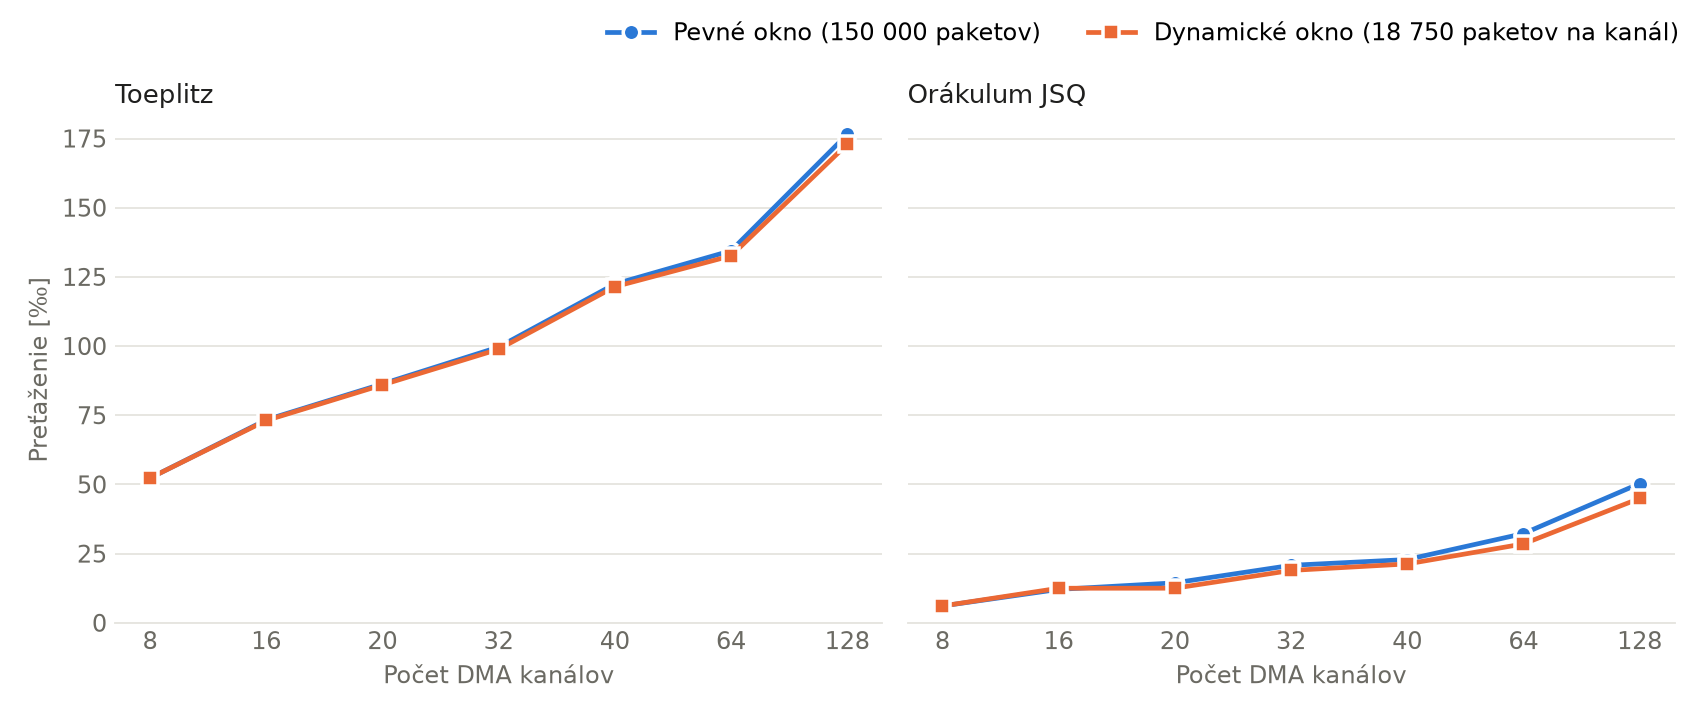
\includegraphics[width=0.9\textwidth]{analyza/pevne_vs_dynamicke_okno.png}
  \caption{Pevné a dynamické okno, váha packet, \texttt{odid1}.}
  \label{fig:okno}
\end{figure}

Pri pevnom okne dostane jeden kanál pri 128 kanáloch 16-krát menej paketov než pri 8.
Mohlo by sa preto zdať, že rast preťaženia s~počtom kanálov je iba artefakt merania.
Tabuľka~\ref{tab:dynamicke-okno} ukazuje, že na \texttt{odid1} to tak \textbf{nie je}: pri
128 kanáloch klesne preťaženie Toeplitzu po prechode na dynamické okno iba zo 176,5 na
172,9\,\textperthousand{} (približne 2\,\%) a orákula z~50,3 na 45,0\,\textperthousand.
Rast preťaženia je teda vlastnosťou prevádzky, nie dĺžky okna.

\emph{Poznámka:} na malom syntetickom datasete (\texttt{flow\_big}, približne 883 súbežných
smerov tokov) bol vplyv okna oveľa väčší (662 oproti 391\,\textperthousand). Výsledok preto
závisí od počtu súbežných tokov a treba ho overiť na ďalších vzorkách.

\section{Ďalšie vzorky prevádzky}
\label{sec:dalsie-vzorky}

Porovnanie funkcií prebehlo aj na vzorkách \texttt{odid2}, \texttt{odid4} a \texttt{odid6} a na
\texttt{odid1} s~hashovaním iba IP adries. Všetky grafy sú v~prílohe~\ref{app:grafy}.

\textbf{Pozor na rozdiely oproti predošlým sekciám:} tieto behy pochádzajú zo staršej verzie
kódu a namiesto jednoduchej tabelácie obsahujú multiply-shift (NH). Surové výsledky sa neuložili,
preto sú čísla v~tabuľke~\ref{tab:vzorky} iba \emph{orientačne odčítané z~grafov}.
\TODO{Prepočítať novým simulátorom a nahradiť presnými hodnotami.}

\begin{table}[ht]
  \centering
  \small
  \caption{Toeplitz na rôznych vzorkách, váha \texttt{packet}, bez symetrie, pevné okno.
  Okrem \texttt{odid1} (plný tuple) sú hodnoty orientačne odčítané z~grafov.}
  \label{tab:vzorky}
  \begin{tabular}{l r r l}
    \toprule
    Vzorka & 8 kanálov [\textperthousand] & 128 kanálov [\textperthousand] & Najväčšia odchýlka funkcie od Toeplitzu \\
    \midrule
    \texttt{odid1} (plný tuple) & 52   & 177  & 7\,\% (Chaskey, lepší) \\
    \texttt{odid2}              & 70   & 240  & 7,5\,\% (multiply-shift, horší) \\
    \texttt{odid4}              & 185  & 525  & 1,6\,\% (multiply-shift, lepší) \\
    \texttt{odid6}              & 115  & 280  & 1,3\,\% \\
    \texttt{odid1} (iba IP)     & 65   & 220  & 12\,\% (multiply-shift, horší) \\
    \bottomrule
  \end{tabular}
\end{table}

Z~porovnania vzoriek vyplývajú tri pozorovania:

\begin{enumerate}
  \item \textbf{Úroveň preťaženia závisí od prevádzky.} Medzi vzorkami sa líši približne
        3,5-násobne (pri 8 kanáloch 52 až 185\,\textperthousand). Rast s~počtom kanálov majú
        všetky vzorky.
  \item \textbf{Kvalitné funkcie zostávajú blízko seba.} Toeplitz, jhash, Chaskey a HalfSipHash
        sa pri váhe \texttt{packet} líšia najviac o~jednotky percent na každej vzorke.
  \item \textbf{Slabšia funkcia sa môže prejaviť pri vstupe s~nízkou entropiou.} Pri hashovaní iba IP
        adries je multiply-shift horší než Toeplitz konzistentne pri všetkých počtoch kanálov:
        približne o~6--12\,\% (packet), 6--11\,\% (byte) a 4--16\,\% (flow). Menší náznak je aj
        na \texttt{odid2} (do 7,5\,\%). Výber hashu teda nie je úplne ľubovoľný.
        \TODO{Príčinu (nízka entropia vstupu) sme zatiaľ neoverili, je to hypotéza.}
\end{enumerate}

\begin{figure}[ht]
  \centering
  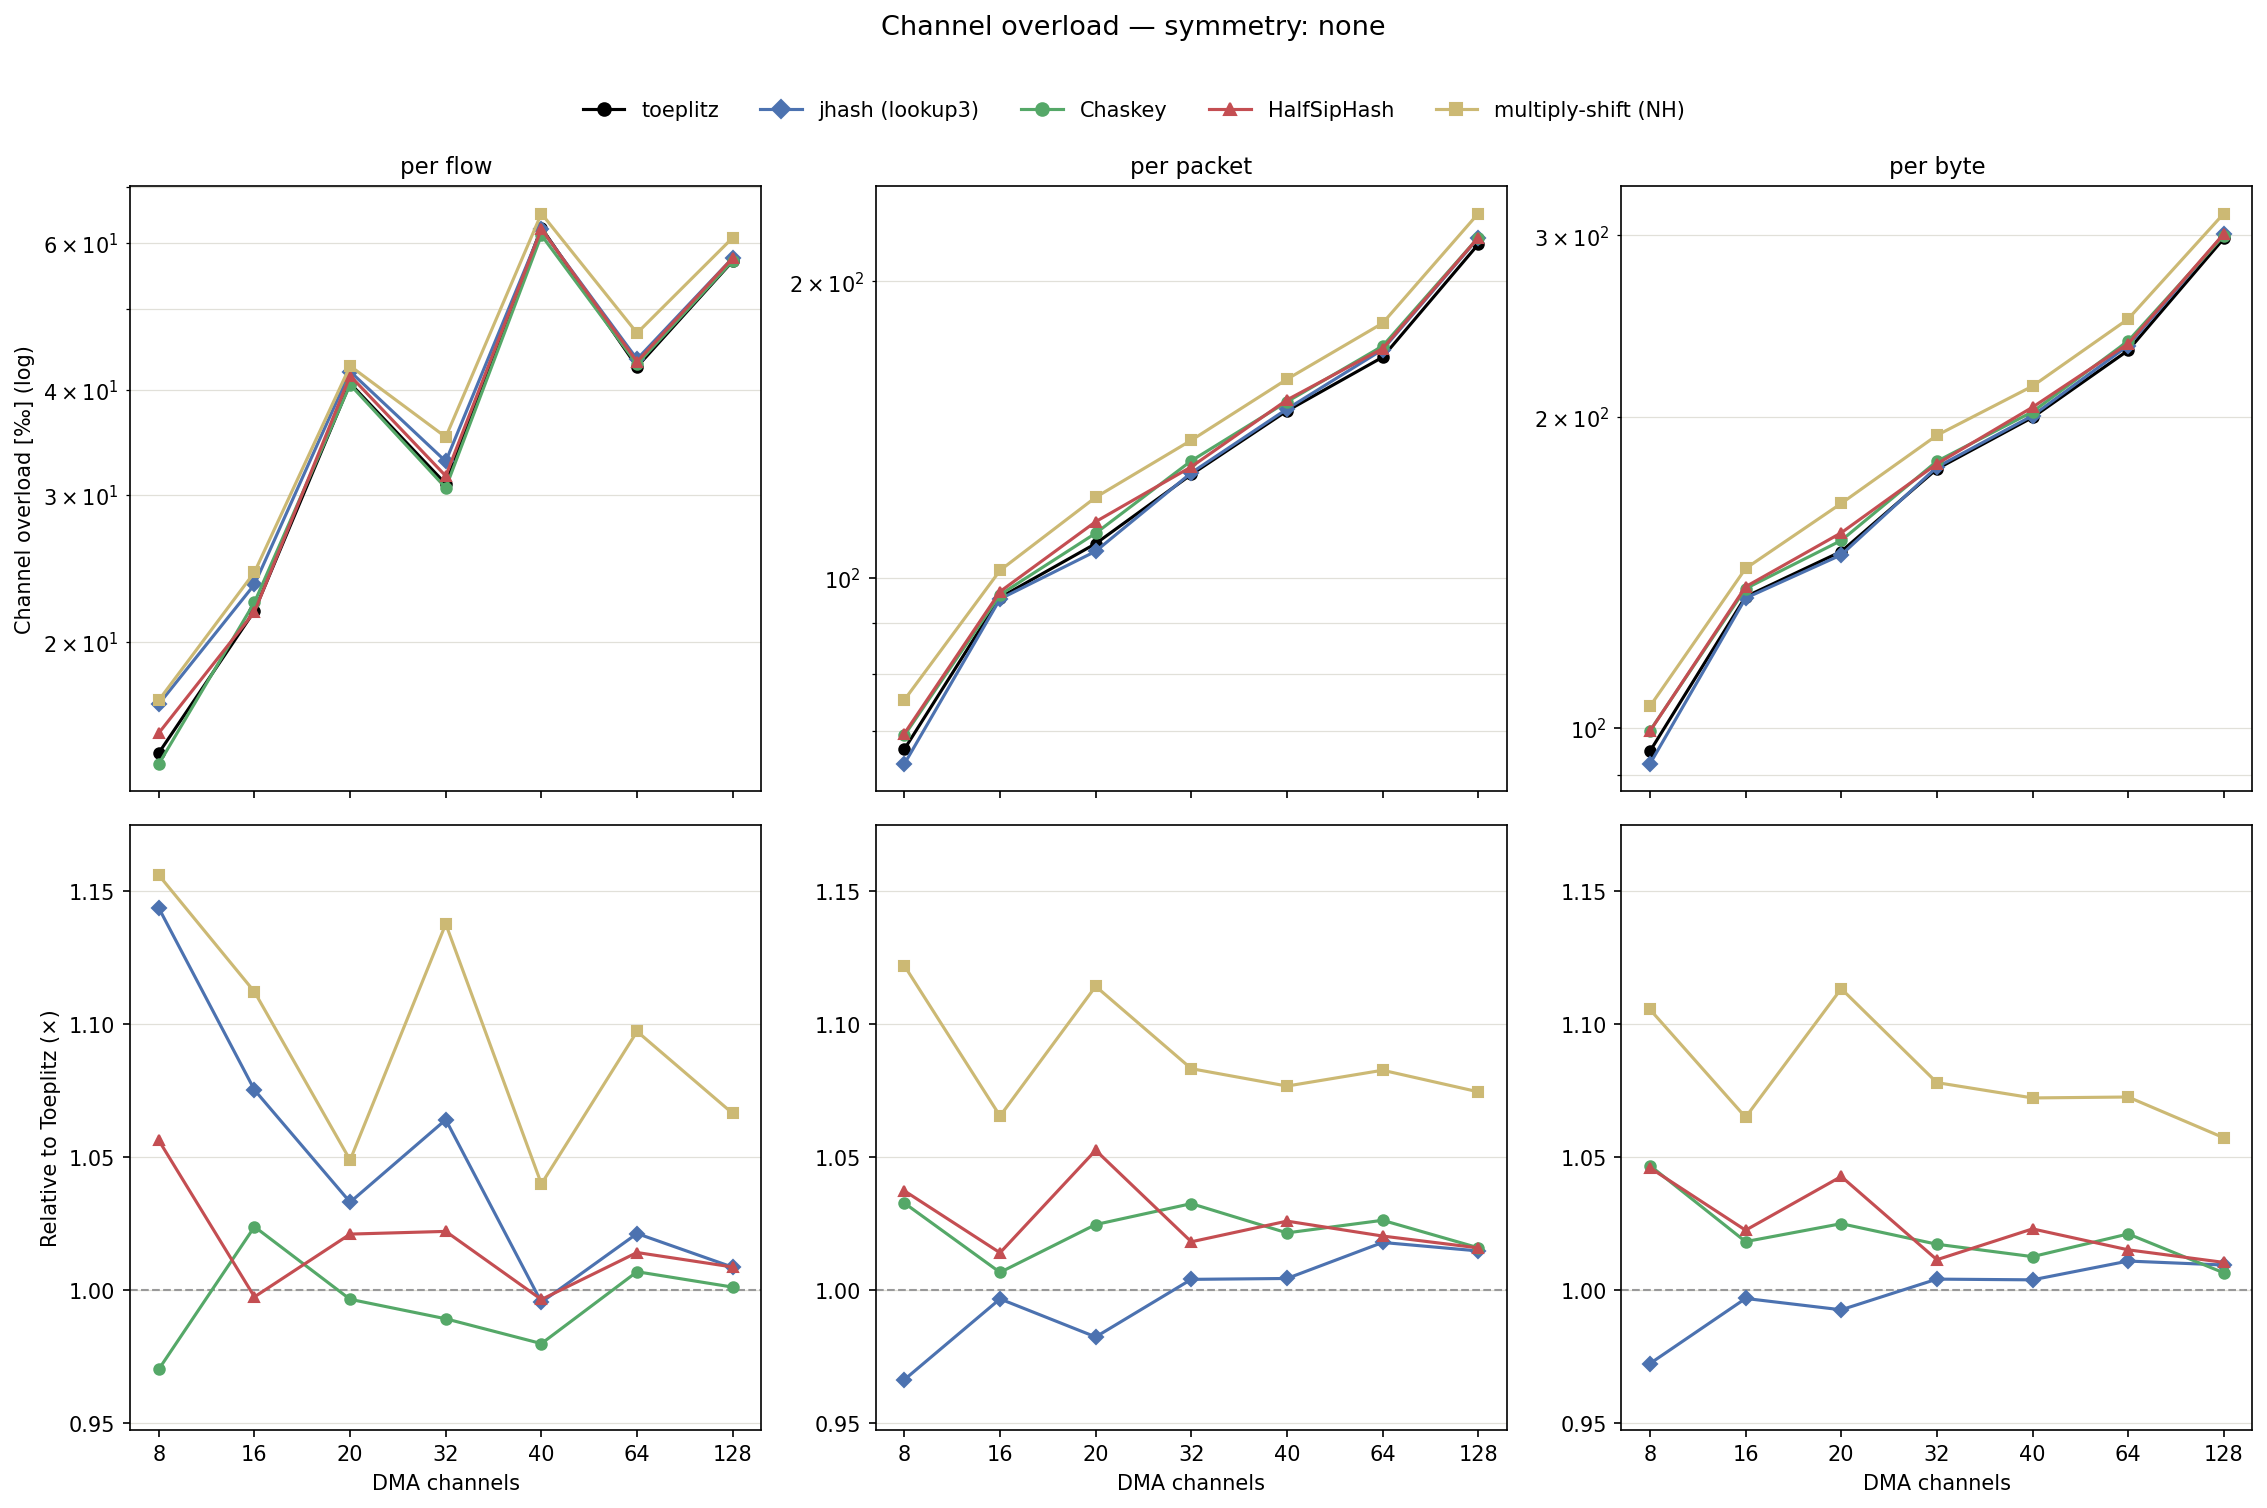
\includegraphics[width=\textwidth]{ostatne_vzorky/odid1_ip_only/overload_none.png}
  \caption{Hashovanie iba IP adries, \texttt{odid1}, staršia verzia kódu s~funkciou multiply-shift.
  V~spodnom riadku je vidno, že multiply-shift je pri všetkých váhach nad Toeplitzom.}
  \label{fig:ip-only}
\end{figure}

Hashovanie iba IP adries navyše zvyšuje samotné preťaženie: pri 128 kanáloch a váhe \texttt{flow}
je približne 57\,\textperthousand{} oproti 19,0\,\textperthousand{} pri plnom tuple
(obrázok~\ref{fig:ip-only}), lebo všetky toky medzi tou istou dvojicou adries skončia v~jednom kanáli.

\section{Zhrnutie}

\begin{enumerate}
  \item Nerovnomernú záťaž spôsobuje rozdielna veľkosť tokov, nie kvalita hashu.
  \item Medzi kvalitnými hashmi sa nepreukázal rozdiel väčší než vplyv kľúča. Slabá funkcia
        (multiply-shift) však môže byť horšia pri vstupe s~nízkou entropiou.
  \item Kľúč má pri malom počte kanálov veľký vplyv: pri 8 kanáloch 42 až 71\,\textperthousand.
  \item Symetria stojí 14--18\,\% pri váhach flow a packet, 2--4\,\% pri bajtoch.
  \item Pri počtoch kanálov, ktoré nedelia 128, pridáva preťaženie aj tabuľka RETA.
  \item Lepší výber kanála pri zachovaní afinity by mohol odstrániť 63--88\,\% preťaženia.
  \item Dĺžka okna výsledky na \texttt{odid1} takmer nemení.
\end{enumerate}
